\chapter{Tracce d'esame}
\section{Esame del 16 gennaio 2023}
\begin{center}
	\includegraphics[scale=.85]{pdf/23-01-16.pdf}
\end{center}
\subsection*{Esercizio 1}
La tautologia della negazione dell'implicazione afferma che sono equivalenti le seguenti proposizioni:
\begin{align*}
	\neg(\alpha \implies \beta) \iff (\alpha \land \neg \beta)
\end{align*}
Infatti, sfruttando la tautologia dell'implicazione come disgiunzione abbiamo:
\begin{align*}
	\neg \bigl(\alpha \implies \beta \bigr) &\iff \neg \bigl( \neg \alpha \lor \beta \bigr) \\
	&\iff \neg (\neg \alpha) \land \neg \beta & \text{\textcolor{gray}{(Applicando la legge di De Morgan)}} \\
	&\iff \alpha \land \neg(\beta)
\end{align*}
Sfruttando questa tautologia allora abbiamo:
\begin{align*}
	\neg \biggl(\exists x \Bigl(\forall y \bigl( f(x,y) \implies g(x,y) \bigr)\Bigr)\biggr) &\iff \forall x \Bigl( \exists y \bigl( f(x,y) \land \neg g(x,y) \bigr)\Bigr)
\end{align*}
\subsection*{Esercizio 2}
\begin{enumerate}[label=(\textit{\roman*})]
	\item $|T|=|A|^{|A|}$ e $|S|=|A|^{|B|}$;
	\item \begin{enumerate}[label=(\alph*)]
		\item Sia $f$ iniettiva e supponiamo che $r(f)$ non sia iniettiva. Allora esistono $x,y \in B$ tali che $r(f)(x) =r(f)(y)$ e $x \neq y$. Ma, per definizione di restrizione, $r(f)(x) = f(x)$ e $r(f)(y)=f(y)$, quindi esistono $x,y \in A$ tali che $f(x)=f(y)$, il che va contro l'ipotesi che $f$ sia iniettiva. Quindi $r(f)$ non può non essere iniettiva se $f$ è iniettiva e l'implicazione risulta vera.
		\item Analogamente, sia $f$ suriettiva e supponiamo $r(f)$ non suriettiva. Ciò implica che esiste un $x \in A$ tale che $\overleftarrow{r(f)}(\{x\})=\emptyset$, ovvero non esiste $y \in B$ (e quindi di $A$) tale che $r(f)(y)=f(y)=x$. Quindi $f$ non risulterebbe suriettiva, contro le nostre ipotesi. Quindi, come nel punto precedente, si ha la veridicità dell'implicazione.
	\end{enumerate}
\item Essendo $|T| \geq |S|$ non possono esistere applicazioni iniettive da $T$ in $S$, quindi $r$ in particolare non può essere iniettiva. Infatti possono esistere applicazioni distinte da $A$ in $A$ che ammettono la stessa restrizione. Al contrario, per ogni restrizione è possibile costruire un prolungamento, per cui $r$ risulta essere una applicazione suriettiva.
\item Abbiamo:
\begin{align*}
	[h]_{\mathfrak{R}} &= \{ f \in T \; | \; r(f) = r(h)\} \\
	&= \{ f \in T \; | \; \forall x \in B (r(f)(x) = 3)\}
\end{align*}
Quindi in $[h]_{\mathfrak{R}}$ sono presenti le funzioni $f_{i}$ costruite ponendo:
\begin{align*}
	f_{i}: x \in A \mapsto \begin{cases*}
		3 & \iff x \in B \\
		i & \iff x \in A \setminus B = \{10\}
	\end{cases*}
\end{align*}
con $i$ che varia in $\{1,...,10\}$, per $i=3$ otteniamo proprio $h$. Quindi $|[h]_{\mathfrak{R}}| = 10$. Per il Teorema \ref{thm:teor_omomorfismo} abbiamo che $|T/{\mathfrak{R}}|=| im \ r| = |S|$ in quanto abbiamo detto che $r$ è suriettiva.
\end{enumerate}
\subsection*{Esercizio 3}
\begin{enumerate}[label=(\textit{\roman*})]
	\item Consideriamo la relazione di divisibilità in $\mathbb{Z}_{9}$, otteniamo il seguente diagramma di Hasse:
	\begin{center}
		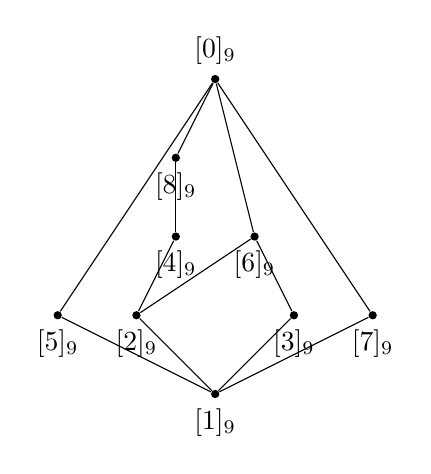
\begin{tikzpicture}
			\node[circle,fill=black,inner sep=0pt,minimum size=3pt,label=below:{$[1]_{9}$}](1) at (0,0){};
			\node[circle,fill=black,inner sep=0pt,minimum size=3pt,label=below:{$[5]_{9}$}](5) at (-2,1){};
			\node[circle,fill=black,inner sep=0pt,minimum size=3pt,label=below:{$[3]_{9}$}](3) at (1,1){};
			\node[circle,fill=black,inner sep=0pt,minimum size=3pt,label=below:{$[4]_{9}$}](4) at (-0.5,2){};
			\node[circle,fill=black,inner sep=0pt,minimum size=3pt,label=below:{$[2]_{9}$}](2) at (-1,1){};
			\node[circle,fill=black,inner sep=0pt,minimum size=3pt,label=below:{$[6]_{9}$}](6) at (0.5,2){};
			\node[circle,fill=black,inner sep=0pt,minimum size=3pt,label=below:{$[7]_{9}$}](7) at (2,1){};
			\node[circle,fill=black,inner sep=0pt,minimum size=3pt,label=below:{$[8]_{9}$}](8) at (-0.5,3){};
			\node[circle,fill=black,inner sep=0pt,minimum size=3pt,label=above:{$[0]_{9}$}](0) at (0,4){};
			\draw[thin,black] (1)--(5);
			\draw[thin,black] (1)--(2);
			\draw[thin,black] (1)--(3);
			\draw[thin,black] (1)--(7);
			\draw[thin,black] (2)--(4);
			\draw[thin,black] (2)--(6);
			\draw[thin,black] (3)--(6);
			\draw[thin,black] (4)--(8);
			\draw[thin,black] (5)--(0);
			\draw[thin,black] (8)--(0);
			\draw[thin,black] (6)--(0);
			\draw[thin,black] (7)--(0);
		\end{tikzpicture}
	\end{center}
Portandoci su $(\mathbb{Z},\rho)$ osserviamo che ogni classe di resto contiene infiniti interi:
\begin{align*}
	[n]_{9} = \{ z \in \mathbb{Z} \; | \; \exists k \in \mathbb{Z}(z = 9k +n)\}
\end{align*}
Dal diagramma di Hasse disegnato si osserva che gli interi appartenenti alla classe di 1 modulo 9 risultano essere minimali in $(\mathbb{Z},\rho)$. Analogamente, gli interi appartenenti alla classe di 0 modulo 9 (i multipli di 9) risultano essere massimali in $(\mathbb{Z},\rho)$. Poiché due elementi appartenenti alla stessa classe sono in relazione $\rho$ se e solo se essi coincidono abbiamo che due elementi distinti nella stessa classe di resto risultano essere inconfrontabili e quindi non esiste un minimo ed un massimo in $(\mathbb{Z},\rho)$.
\item Osserviamo che sia $127 \in [1]_{9}$ che $721 \in [1]_{9}$\footnote{Basta applicare i criteri di divisibilità.}. Quindi i due elementi sono inconfrontabili, essendo $[1]_{9}$ il minimo in $(\mathbb{Z}_{9},\divides)$ non esistono minoranti di $\{127,721\}$ mentre esistono infiniti interi, a due a due inconfrontabili, maggioranti di $\{127,721\}$, quindi non esiste neanche un estremo superiore.
\item Per i motivi esposti al punto precedente $(\mathbb{Z},\rho)$ non risulta essere un reticolo.
\item Osservando il diagramma di Hasse di $(\mathbb{Z}_{9},\divides)$ osserviamo che è possibile individuare una catena massimale considerando le classi $[1]_{9}, \ [2]_{9}, \ [4]_{9}, \ [8]_{9}, \ [0]_{9}$. Spostandoci in $(\mathbb{Z},\rho)$ e prendendo un singolo elemento di ciascuna classe si ottiene un sottoinsieme massimale (rispetto all'inclusione). Ad esempio:
\begin{displaymath}
	\{10,11,13,17,18\}
\end{displaymath}
\item Abbiamo:
\begin{itemize}
	\item $-90 \in [0]_{9}$
	\item $-15 \in [3]_{9}$
	\item $-3 \in [6]_{9}$
	\item $7 \in [7]_{9}$
	\item $15 \in [6]_{9}$
	\item $94 \in [4]_{9}$
	\item $100 \in [1]_{9}$
\end{itemize}
Otteniamo così il seguente diagramma di Hasse:
\begin{center}
	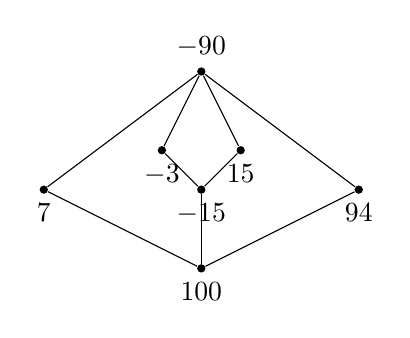
\begin{tikzpicture}
		\node[circle,fill=black,inner sep=0pt,minimum size=3pt,label=below:{$100$}](a) at (0,0){};
		\node[circle,fill=black,inner sep=0pt,minimum size=3pt,label=below:{$7$}](b) at (-2,1){};
		\node[circle,fill=black,inner sep=0pt,minimum size=3pt,label=below:{$-15$}](c) at (0,1){};
		\node[circle,fill=black,inner sep=0pt,minimum size=3pt,label=below:{$94$}](d) at (2,1){};
		\node[circle,fill=black,inner sep=0pt,minimum size=3pt,label=below:{$15$}](e) at (0.5,1.5){};
		\node[circle,fill=black,inner sep=0pt,minimum size=3pt,label=below:{$-3$}](f) at (-0.5,1.5){};
		\node[circle,fill=black,inner sep=0pt,minimum size=3pt,label=above:{$-90$}](g) at (0,2.5){};
		\draw[thin,black] (a)--(b);
		\draw[thin,black] (a)--(c);
		\draw[thin,black] (a)--(d);
		\draw[thin,black] (c)--(e);
		\draw[thin,black] (c)--(f);
		\draw[thin,black] (d)--(g);
		\draw[thin,black] (b)--(g);
		\draw[thin,black] (e)--(g);
		\draw[thin,black] (f)--(g);
	\end{tikzpicture}
\end{center}
Tale insieme ordinato è un reticolo complementato, ma non è distributivo in quanto il sottoreticolo: $$(\{100,7,-15,94,-90\},\rho)$$ è isomorfo al reticolo trirettangolo:
\begin{center}
	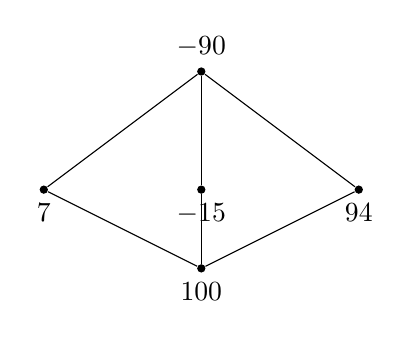
\begin{tikzpicture}
		\node[circle,fill=black,inner sep=0pt,minimum size=3pt,label=below:{$100$}](a) at (0,0){};
		\node[circle,fill=black,inner sep=0pt,minimum size=3pt,label=below:{$7$}](b) at (-2,1){};
		\node[circle,fill=black,inner sep=0pt,minimum size=3pt,label=below:{$-15$}](c) at (0,1){};
		\node[circle,fill=black,inner sep=0pt,minimum size=3pt,label=below:{$94$}](d) at (2,1){};
		\node[circle,fill=black,inner sep=0pt,minimum size=3pt,label=above:{$-90$}](g) at (0,2.5){};
		\draw[thin,black] (a)--(b);
		\draw[thin,black] (a)--(c);
		\draw[thin,black] (a)--(d);
		\draw[thin,black] (c)--(g);
		\draw[thin,black] (d)--(g);
		\draw[thin,black] (b)--(g);
	\end{tikzpicture}
\end{center}
\end{enumerate}
\subsection*{Esercizio 4}
\begin{enumerate}[label=(\textit{\roman*})]
	\item L'operazione $\ast$ risulta essere associativa e commutativa. Infatti:
	\begin{align*}
		\forall x,y \in \mathbb{Z}_{16} \bigl( x \ast y = 3xy = 3yx = y \ast x \bigr)
	\end{align*}
Inoltre, presi $a,b,c \in \mathbb{Z}_{16}$ abbiamo:
\begin{align*}
	a \ast (b \ast c ) = a \ast (3bc) = 3a(3bc) = 9abc \\
	(a \ast b) \ast c = (3ab) \ast c = 3(3ab)c = 9abc
\end{align*}
Un elemento $t \in \mathbb{Z}_{16}$ è neutro in $(\mathbb{Z}_{16},\ast)$ se e solo se, per ogni $a \in \mathbb{Z}_{16}$ risulta:
\begin{align*}
	a \ast t = t \ast a  = 3ta = a &\iff 3t \equiv_{16} 1 \\
	&\iff t = \overline{11}
\end{align*}
Quindi $t= \overline{11}$ è il neutro del monoide $(\mathbb{Z}_{16},\ast)$. Un elemento $a \in \mathbb{Z}_{16}$ ammette simmetrico se e solo se esiste un $a' \in \mathbb{Z}_{16}$ tale che $a \ast a' = 11$, ovvero:
\begin{align*}
	3aa' \equiv_{16} 11 &\iff aa' \equiv_{16} 9 & \text{\textcolor{gray}{(Moltiplicando per 11 inverso di 3)}}
\end{align*}
Tale equazione ammette soluzione se e solo se $(a,16) \divides 9$. I divisori di $16$ minori di 9 sono $1, \ 2, \ 4, \ 8$ e solo divide 9. Possiamo concludere che se $a \in \{1,3,5,7,9\}$ allora $(a,16)=1 \divides 9$. Troviamo l'inverso di $x=\overline{1}$:
\begin{align*}
	x \ast x' \equiv_{16} 11 &\iff 3x' \equiv_{16} 11 \\
	&\iff x' \equiv_{16} 9
\end{align*}
	\item Risulta $7 \ast 7 = 3 \cdot 49 = 3 \cdot 1 = 3 \notin H$, quindi $H$ non è stabile in $(\mathbb{Z}_{16},\ast)$
	\item Un elemento $a \in \mathbb{Z}_{16}$ è divisore dello zero in $(\mathbb{Z}_{16},+,\ast)$ se esiste un elemento $b \in \mathbb{Z}_{16} \setminus \{\overline{0}\}$ tale che $ a \ast b=\overline{0}$. Abbiamo:
	\begin{align*}
		a \ast b = 3ab = \overline{0}
	\end{align*}
Essendo $3$ coprimo con $16$ abbiamo che tale elemento è simmetrizzabile e quindi cancellabile, per rendere il prodotto nullo abbiamo quindi bisogno che $ab = \overline{0}$. Tale richiesta si traduce quindi nella ricerca dei divisori dello zero in $(\mathbb{Z}_{16},\cdot)$ i quali sono tutti e soli gli elementi non invertibili, cioè $\mathbb{Z}_{16} \setminus \mathcal{U}(\mathbb{Z}_{16}) = \{0,2,4,6,8,10,12,14\}$.
\end{enumerate}
\subsection*{Esercizio 5}
Un circuito euleriano in un grafo è un percorso chiuso che attraversa ciascun arco del grafo esattamente una volta. Perché un grafo possa ammettere un circuito euleriano, deve soddisfare due condizioni:
\begin{itemize}
	\item Tutti i vertici devono avere grado pari
	\item Il grafo deve essere connesso
\end{itemize}
Un grafo completo $K_{n}$​ è un grafo in cui ogni coppia di vertici è connessa da un arco, quindi in particolare è un grafo connesso. Per un grafo completo, il grado di ogni vertice è $n−1$, poiché ogni vertice è collegato a tutti gli altri $n−1$ vertici. Quindi se $n-1$ deve essere pari ciò significa che $n$ è un numero dispari. Quindi ogni grafo completo con un numero dispari di vertici ammette circuiti euleriani.
\subsection*{Esercizio 6}
\begin{enumerate}[label=(\textit{\roman*})]
	\item Applicando il Criterio di Eisenstein con $p=2$ abbiamo che $2$ divide i coefficienti $a_{0},...,a_{3}$, 2 non divide $a_{n}=4$ e $p^{2}=4$ non divide 2. Quindi il polinomio $f$ è irriducibile in $\mathbb{Q}$ e di conseguenza, essendo associato al polinomio $f_{1} \in \mathbb{Z}_{1}[x] = \mathbb{Z}[x]$, è irriducibile anche in $\mathbb{Z}[x]$.
	\item Risulta $f_{5} = 4x+2$. Per trovare un polinomio monico associato risolviamo l'equazione $4x \equiv{5} 1$ che ha soluzione per $x=4$, quindi moltiplicando $f_{5}$ per 4 otteniamo:
	\begin{align*}
		4 \cdot f_{5} &= 4 \cdot (4x+2)   \\
		&= 16x + 8 \\
		&= x + 3
	\end{align*}
Analogamente, per $f_{32}$ risolviamo l'equazione $5x \equiv_{32} 1$ ottenendo $x=13$. Moltiplichiamo quindi $f_{32}$ per $x=\overline{13}$:
\begin{align*}
	13 \cdot f_{32} &= 13 \cdot \bigl(5x^{4} + 10x^{2}+4x+2\bigr) \\
	&= x^{4} +2x^{2} +20x + 26
\end{align*}
\item Un polinomio è cancellabile se e solo se $cd(f)$ è cancellabile nell'anello dei coefficienti. In questo caso, essendo $cd(f)=5$ un numero primo abbiamo che per ogni intero non nullo $n <10$ 5 è coprimo con $n$ e quindi simmetrizzabile, quindi cancellabile.
\end{enumerate}
\vfill
\section{Esame del 13 luglio 2023}
\begin{center}
	\includegraphics[scale=.85]{pdf/23-07-13.pdf}
\end{center}
\subsection*{Esercizio 1}
Abbiamo:
\begin{enumerate}[label=(\textit{\roman*})]
	\item \textbf{Falso}. L'insieme vuoto non è un elemento del singleton del singleton dell'insieme vuoto ma è tutt'al più una sua parte.
	\item \textbf{Falso}. Non ha senso confrontare un numero cardinale con un insieme. Il simbolo $|\mathbb{N}|$ indica infatti la cardinalità di $\mathbb{N}$, ovvero il numero dei suoi elementi, che è quantificabile col simbolo $\aleph$. Il simbolo $\{\mathbb{N}\}$ indica invece il singleton dell'insieme dei numeri naturali.
	\item \textbf{Vera}. Notiamo infatti che l'antecedente risulta essere una proposizione falsa in quanto l'insieme dei tre elementi $\{1,2,3\}$ non è uguale all'insieme $\{3!\}=\{6\}$. L'implicazione risulta quindi essere vera in quanto l'antecedente è falsa.
	\item \textbf{Vera}. Una applicazione $f: \{1,2\} \rightarrow \mathbb{N}$ è un'applicazione per la quale $\forall x \in \{1,2\}$  esiste un $n \in \mathbb{N}$ tale che $n=f(x)$. Il grafico $\{(1,1),(2,1)\}$ descrive in particolare l'applicazione costante $c_{1}$ che associa l'elemento 1 ad ogni elemento dell'insieme $\{1,2\}$.
\end{enumerate}
\subsection*{Esercizio 2}
L'insieme $S = \mathbb{N} \cap [0]_{3}$ è l'insieme dei multipli di $3$, ovvero:
\begin{align*}
	S =  \mathbb{N} \cap [0]_{3} = \{n \in \mathbb{N} \; | \; \exists k \in \mathbb{N} (n=3k)\} = 3\mathbb{N}
\end{align*}
L'applicazione caratteristica $\text{\Large\chi}_{\mathbb{N},S}$ restituisce 1 se $n \in 3\mathbb{N}$, 0 altrimenti. In particolare, $\forall n \in \mathbb{N}$:
\begin{align}\label{eq:130723_20}
	n^{\chi(a)} = 
	\begin{cases}
		a^{1} &\iff a \in 3\mathbb{N} \\
		a^{0} &\iff a \notin 3\mathbb{N}
	\end{cases}
\end{align}
\begin{enumerate}[label=(\textit{\roman*})]
	\item L'operazione $\ast$ è banalmente commutativa in quanto lo è la moltiplicazione ordinaria in $\mathbb{N}$. Per verificare l'associatività bisogna verificare che per ogni terna numerica $(a,b,c)$ di elementi di $\mathbb{N}$ risulti:
	\begin{align*}
		(a \ast b) \ast c = a \ast (b \ast c)
	\end{align*}
	Sviluppando il membro a sinistra otteniamo:
	\begin{align}
		(a \ast b) \ast c &= \bigl(a^{\chi(a)} \cdot b^{\chi(b)} \bigr) \ast c \nonumber \\
		&= \bigl( a^{\chi(a)} \cdot b^{\chi(b)}\bigr)^{\chi(a^{\chi(a)} \cdot b^{\chi(b)})} \cdot c^{\chi(c)} \label{eq:130723_21}
	\end{align}
	Mentre, sviluppando il membro a destra:
	\begin{align}
		a \ast (b \ast c) &= (b \ast c) \ast a & \text{\textcolor{gray}{(Applicando la commutatività di $\ast$)}} \nonumber \\
		&= \bigl(b^{\chi(b)}\cdot c^{\chi(c)}\bigr)^{\chi(b^{\chi(b)} \cdot c^{\chi(c)})} \cdot a^{\chi(a)} \label{eq:130723_22}
	\end{align}
	La verifica dell'uguaglianza di \ref{eq:130723_21} con \ref{eq:130723_22} deve essere fatta per casi:
	\begin{enumerate}
		\item Supponiamo il caso in cui $a,b,c \in 3\mathbb{N}$, in questo caso, applicando quanto osservato in \ref{eq:130723_20} otteniamo:
		\begin{align*}
			(a \ast b) \ast c &= \bigl( a^{\chi(a)} \cdot b^{\chi(b)}\bigr)^{\chi(a^{\chi(a)} \cdot b^{\chi(b)})} \cdot c^{\chi(c)} & \text{\textcolor{gray}{
					(Osservando che $ab \in 3\mathbb{N}$)}}\\
			&= (a\cdot b) \cdot c = (ab)c 
		\end{align*}
		e analogamente:
		\begin{align*}
			a \ast (b \ast c) &= \bigl(b^{\chi(b)}\cdot c^{\chi(c)}\bigr)^{\chi(b^{\chi(b)} \cdot c^{\chi(c)})} \cdot a^{\chi(a)} \\
			&= (b \cdot c) \cdot a = a(bc)
		\end{align*}
		\item Siano ora $a,b,c \notin 3\mathbb{N}$. Allora:
		\begin{align*}
			(a \ast b) \ast c = (1 \cdot 1)^{0} \cdot 1 = 1 \\
			(a \ast b) \ast c =  (1 \cdot 1)^{0} \cdot 1 = 1
		\end{align*}
		\item Sia uno tra $a,b,c$ non appartenente a $3\mathbb{N}$. Senza ledere di generalità, sia esso $c$. Abbiamo quindi:
		\begin{align*}
			(a \ast b) \ast c = (a \cdot b) ^{1} \cdot 1 = ab \\
			a \ast (b \ast c) = a(b \cdot 1)^{1} = ab
		\end{align*}
		\item Siano due elementi non appartenenti a $3\mathbb{N}$, siano essi $b,c$, allora:
		\begin{align*}
			(a \ast b) \ast c = (a \cdot 1)^{1} = a \\
			a \ast (b \ast c) = a \cdot (1 \cdot 1)^{0} = a
		\end{align*}
	\end{enumerate}
	In ogni caso il membro a destra e a sinistra coincidono e quindi $\ast$ risulta associativa.
	\item Per esistere elemento neutro rispetto all'operazione $\ast$ deve esistere un $t \in \mathbb{N}$ tale che, per ogni $n \in \mathbb{N}$, garantisca che $n \ast t = t \ast n = n$. Un tale $t$ non può esistere in quanto:
	\begin{align*}
		\forall n \in \mathbb{N} \bigl(n \ast t = n &\iff n^{\chi(n)} \cdot t^{\chi(t)} = n \\
		&\iff n^{\chi(n)} = n \land t^{\chi(t)}=1 \\
		&\iff (n \in 3\mathbb{N}) \land (t \notin 3\mathbb{N}) \bigr)
	\end{align*}
	Dato che non può esistere un tale $t$ che sia neutro per ogni naturale possiamo concludere affermando la sua non esistenza.
	\item Abbiamo $T=2\mathbb{N}$ e $U=\{n \in \mathbb{N} \; | \; \exists k \in \mathbb{N}(n=3k+2)\}$. Una parte $X \subseteq \mathbb{N}$ si dice stabile se, e solo se, per ogni $(a,b) \in X \times X$ si abbia $a \ast b \in X$.
	\begin{itemize}
		\item Presi ad esempio $a=14$ e $b=16$ elementi di $T$ abbiamo:
		\begin{align*}
			14 \ast 16 &= 14^{\chi(14)} \cdot 16^{\chi(16)} \\
			&= 14^{0} \cdot 16^{0} = 1 \notin T
		\end{align*}
		Quindi $T$ non è stabile.
		\item Presi $a=5$ e $b=7$ elementi di $U$, abbiamo:
		\begin{align*}
			5 \ast 7 &= 5^{\chi(5)} \cdot 7^{\chi(7)} \\
			&= 1 \notin U
		\end{align*}
		Quindi $U$ non è stabile.
		\item Presi due elementi $a,b \in S$ abbiamo:
		\begin{align*}
			a \ast b = a^{\chi(a)} \cdot b^{\chi(b)} \\
			&= a \cdot b \in S
		\end{align*}
		Quindi il semigruppo $(S,\ast)$ risulta stabile rispetto a $\ast$.
	\end{itemize}
\end{enumerate}
\subsection*{Esercizio 3}
\begin{enumerate}[label=(\textit{\roman*})]
	\item La relazione $\alpha$ coincide con la relazione identica $id_{\mathbb{N}}$ che è una relazione d'ordine. In $(\mathbb{N},\alpha)$ tutti i numeri sono sia minimali che massimali. Non esistono minimo e massimo. Non potendo definire, per ogni coppia di elementi $(n,m)$ l'infimo ed il supremo della parte $\{a,b\}$ l'insieme ordinato non costituisce un reticolo.
	Presa la parte $S=\{1,20,40,400,10000\}$ abbiamo il seguente diagramma di Hasse:
	\begin{center}
		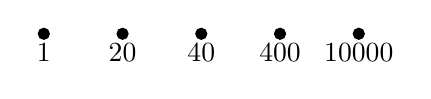
\begin{tikzpicture}
			\filldraw[black] (0,0) circle(2pt) node[anchor=north]{1};
			\filldraw[black] (1,0) circle(2pt) node[anchor=north]{20};
			\filldraw[black] (2,0) circle(2pt) node[anchor=north]{40};
			\filldraw[black] (3,0) circle(2pt) node[anchor=north]{400};
			\filldraw[black] (4,0) circle(2pt) node[anchor=north]{10000};
		\end{tikzpicture}
	\end{center}
	\item  Per verificare che $\beta \in OL(\mathbb{N})$ verifichiamo che essa sia riflessiva, antisimmetrica e transitiva:
	\begin{enumerate}
		\item Chiaramente $\forall a \in \mathbb{N}$ risulta $a \ \beta \ a $ in quanto $a=a$ e questo è sufficiente per garantire la corrispondenza di un numero con se stesso.
		\item Siano $a,b \in \mathbb{N}$ tali che $a \ \beta \ b$ e $b \ \beta \ a$:
		\begin{align}
			\begin{cases}
				a \ \beta \ b &\iff a=b \lor (a \divides b \land a < 10b) \\
				b \ \beta \ a &\iff b=a \lor (b \divides a \land b < 10a)
			\end{cases}
		\end{align}
		Nel caso gli elementi coincidano l'antisimmetria di $\beta$ è una conseguenza triviale. Se $a \divides b \land a <10b$ e $b \divides a \land b<10a$ allora, in particolare, gli elementi risultano essere elementi associati in $\mathbb{N}$ e quindi devono coincidere per forza.
		\item Siano $a,b,c \in \mathbb{N}$ elementi tali che $a \ \beta \ b$ e $b \ \beta \ c$. Allora, se $a=b$ e $b=c$ allora $a=c$ e quindi $ a \ \beta \ c$. Altrimenti, se $a \divides b \land a <10b$ e $b \divides c \land b<10c$ allora possiamo scrivere $b=ka$ per un opportuno $k \in \mathbb{N}$ e $c=mb=m(ka)=a(km)$. Quindi $a \divides c$ e inoltre possiamo eseguire la maggiorazione $a < 10b < 100c$. Quindi vale sicuramente $a < 10c$ e $a \ \beta \ c$. Quindi $\beta \in OL(\mathbb{N})$.	
	\end{enumerate}
	L'elemento 1 risulta essere il minimo in $(\mathbb{N},\beta)$ in quanto, $\forall n \in \mathbb{N}(1 \ \beta \ n)$. Dato che per ogni $a,b$ esiste sempre un elemento $n \in \mathbb{N}$ tale che $n \cdot a > b$, possiamo dire che in  $(\mathbb{N},\beta)$ non esistono elementi massimali e dunque un massimo. L'insieme ordinato risulta essere un reticolo in quanto per ogni parte $\{a,b\}$ possiamo trovare l'infimo ed il supremo che è dato dal massimo comun divisore e dal minimo comune multiplo di $(a,b)$. In particolare $(S,\beta)$ risulta essere un insieme totalmente ordinato. Si ottiene quindi la catena:
	\begin{center}
		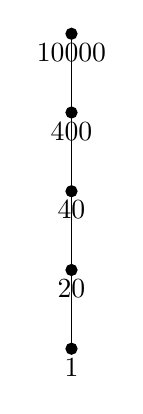
\begin{tikzpicture}
			\filldraw[black] (0,0) circle(2pt) node[anchor=north]{1};
			\filldraw[black] (0,1) circle(2pt) node[anchor=north]{20};
			\filldraw[black] (0,2) circle(2pt) node[anchor=north]{40};
			\filldraw[black] (0,3) circle(2pt) node[anchor=north]{400};
			\filldraw[black] (0,4) circle(2pt) node[anchor=north]{10000};
			\draw[black](0,0)--(0,1)--(0,2)--(0,3)--(0,4);
		\end{tikzpicture}
	\end{center}
	\item La relazione $\gamma$ coincide con la relazione $\alpha$ in quanto osserviamo che la proposizione $(a \divides b \land a > 10b)$ risulta sempre falsa. Infatti un divisore non può essere maggiore di un multiplo dell'elemento che divide. Resta però la condizione di uguaglianza la quale, come visto nel primo punto, risulta essere una relazione d'ordine.
	\item La relazione $\delta$ non risulta essere una relazione d'ordine in $\mathbb{N}$ in quanto non soddisfa la proprietà antisimmetrica. Infatti presi $a,b \in \mathbb{N}$ tali che $a \ndivides b$ e $b \ndivides a$, ovvero $a \ \delta \ b$ e $b \ \delta \ a$, ciò non implica che sia necessariamente $a=b$. Ad esempio abbiamo $2 \ \delta \ 5$ e $5 \ \delta \ 2$ in quanto $2 \ndivides 5$ e $5 \ndivides 2$ ma $2 \neq 5$.
\end{enumerate}

\subsection*{Esercizio 4}
Un grafo si dice connesso se per ogni coppia di vertici esiste un cammino. Se il numero di vertici è pari a 16 ciò significa che devono esistere almeno 15 lati. Per questo motivo non è possibile disegnare un grafo connesso con 16 vertici e 10 lati.
\subsection*{Esercizio 5}
Calcoliamo il Massimo Comun Divisore tra 111 e 126.
\begin{align*}
	111 = 3 \cdot 37 \\
	126 = 2 \cdot 3^{2} \cdot 7
\end{align*}
L'equazione $111n \equiv_{126} 11$ non ammette soluzioni in quanto $MCD(111,126)=3$ non divide 11, mentre $111n \equiv_{126} 12$ risulta essere una equazione compatibile. Dividendo tutti i termini per 3 si ottiene l'equazione equivalente ridotta:
\begin{align*}
	\frac{111}{3}n \equiv_{\frac{126}{3}} \frac{12}{3} = 37n \equiv_{42} 4
\end{align*}
E vale $MCD(37,42)=1$. Cerchiamo una combinazione lineare $37u+42v=1$. Applicando l'algoritmo delle divisioni successive si ottiene:
\begin{align*}
	42 = 37 \cdot 1 + 5 \\
	37 = 5 \cdot 7 + 2 \\
	5 = 2 \cdot 2 + 1 \\
	2 = 1 \cdot 2 + 0
\end{align*}
Da queste relazioni otteniamo:
\begin{align}
	5 = 42 +(-1)37 \\
	2 = 37 +(-7)5 \\
	1 = 5 + (-2)2
\end{align}
Possiamo dunque esprimere 1 come:
\begin{align*}
	1 &= 5 - 4 \\
	&= \bigl(42-37\bigr)+(-2)\bigl(37-35\bigr) \\
	&= 42 - 37 +(-2)37+(14)5 \\
	&= 42+ (-3)37 +(14)\bigl(42+(-1)37\bigr) \\
	&= 42 + (-3)37 + (14)42+(-14)37 \\
	&= (15)42 + (-17)37
\end{align*}
Moltiplicando tale combinazione lineare per 4 si ottiene:
\begin{align*}
	4 = (60)42 + (-68)37
\end{align*}
Quindi $u=[-68]_{42}=[16]_{42}$ è soluzione dell'equazione. L'insieme $A=\{[16]_{42}\}$ e vale $\{a \in A \; | \; 0 \leq a \leq 84\} = \{16,58\}$.
\subsection*{Esercizio 6}
\begin{enumerate}[label=(\textit{\roman*})]
	\item L'insieme $S$ è costituito dai polinomi $f \in \mathbb{Z}_{5}$ di grado 4 tali che $f(\overline{1})=0$. Un polinomio di grado 4 in $\mathbb{Z}_{5}[x]$ può essere scritto come:
	\begin{align*}
		a_{4}x^{4}+a_{3}x^{3}+a_{2}x^{2}+a_{1}x+a_{0}
	\end{align*}
	Con $a_{4} \neq \overline{0}$, altrimenti non sarebbe un polinomio di quarto grado. Imporre che $f(\overline{1})=0$ è equivalente a dire che:
	\begin{align*}
		a_{4}+a_{3}+a_{2}+a_{1}+a_{0} = 0
	\end{align*}
	La domanda della conta degli elementi di $S$ può essere rivista come il conteggio di tutte le possibili combinazioni degli elementi $a_{i}$ con $i \in \mathbb{Z}_{5}$ tali che $\sum_{i=0}^{4} a_{i}=0$ e tale che $a_{4} \neq \overline{0}$.
	Per ciascuno di questi casi, stiamo essenzialmente chiedendo in quanti modi possiamo scegliere $4$ numeri da $\{0, 1, 2, 3, 4\}$ la cui somma sia un valore specifico. Abbiamo quindi:
	\begin{itemize}
		\item Se $a_{4}=1$, deve essere $a_{3}+a_{2}+a_{1}+a_{0}=4$;
		\item Se $a_{4}=2$, deve essere $a_{3}+a_{2}+a_{1}+a_{0}=3$;
		\item Se $a_{4}=3$, deve essere $a_{3}+a_{2}+a_{1}+a_{0}=2$;
		\item Se $a_{4}=4$, deve essere $a_{3}+a_{2}+a_{1}+a_{0}=1$.
	\end{itemize}
	Per ogni caso, il numero di combinazioni con ripetizione di $4$ elementi presi dall'insieme $\mathbb{Z}_{5}$ che diano somma $k$ con $k \in \{4,3,2,1\}$ è dato da:
	\begin{align*}
		\sum_{k=1}^{4} \binom{4+k-1}{i} &= \binom{4+1-1}{1}+\binom{4+2-1}{2}+\binom{4+3-1}{3}+\binom{4+4-1}{4} \\
		&= 4 + 10 + 20 + 35 \\
		&= 69
	\end{align*}
	\item $(S,+)$ è una parte chiusa. Infatti, presi due polinomi $s,q \in S$ allora $s+q$ calcolato in $\overline{1}$ è equivalente a $s(1)+q(1)=0$. $(S,+)$ non risulta essere abeliano in quanto il polinomio nullo non è un polinomio di grado 4.
	\item Osserviamo che per ogni $f \in S\bigl(\varphi(f)= f(\overline{1})=\overline{0}\bigr)$, e $\varphi$ risulta essere una applicazione costante. Quindi $\varphi$ non è iniettiva e non è suriettiva. 
	\item Essendo costante $\varphi$ il suo nucleo di equivalenza coincide con la relazione totale in $S$. Quindi $S/{\sim_{\varphi}} = S/{\tau_{S}} = \{S\}$, ed esiste un'unica classe di equivalenza.
\end{enumerate}
\vfill

\section{Esame del 15 gennaio 2024}
\begin{center}
	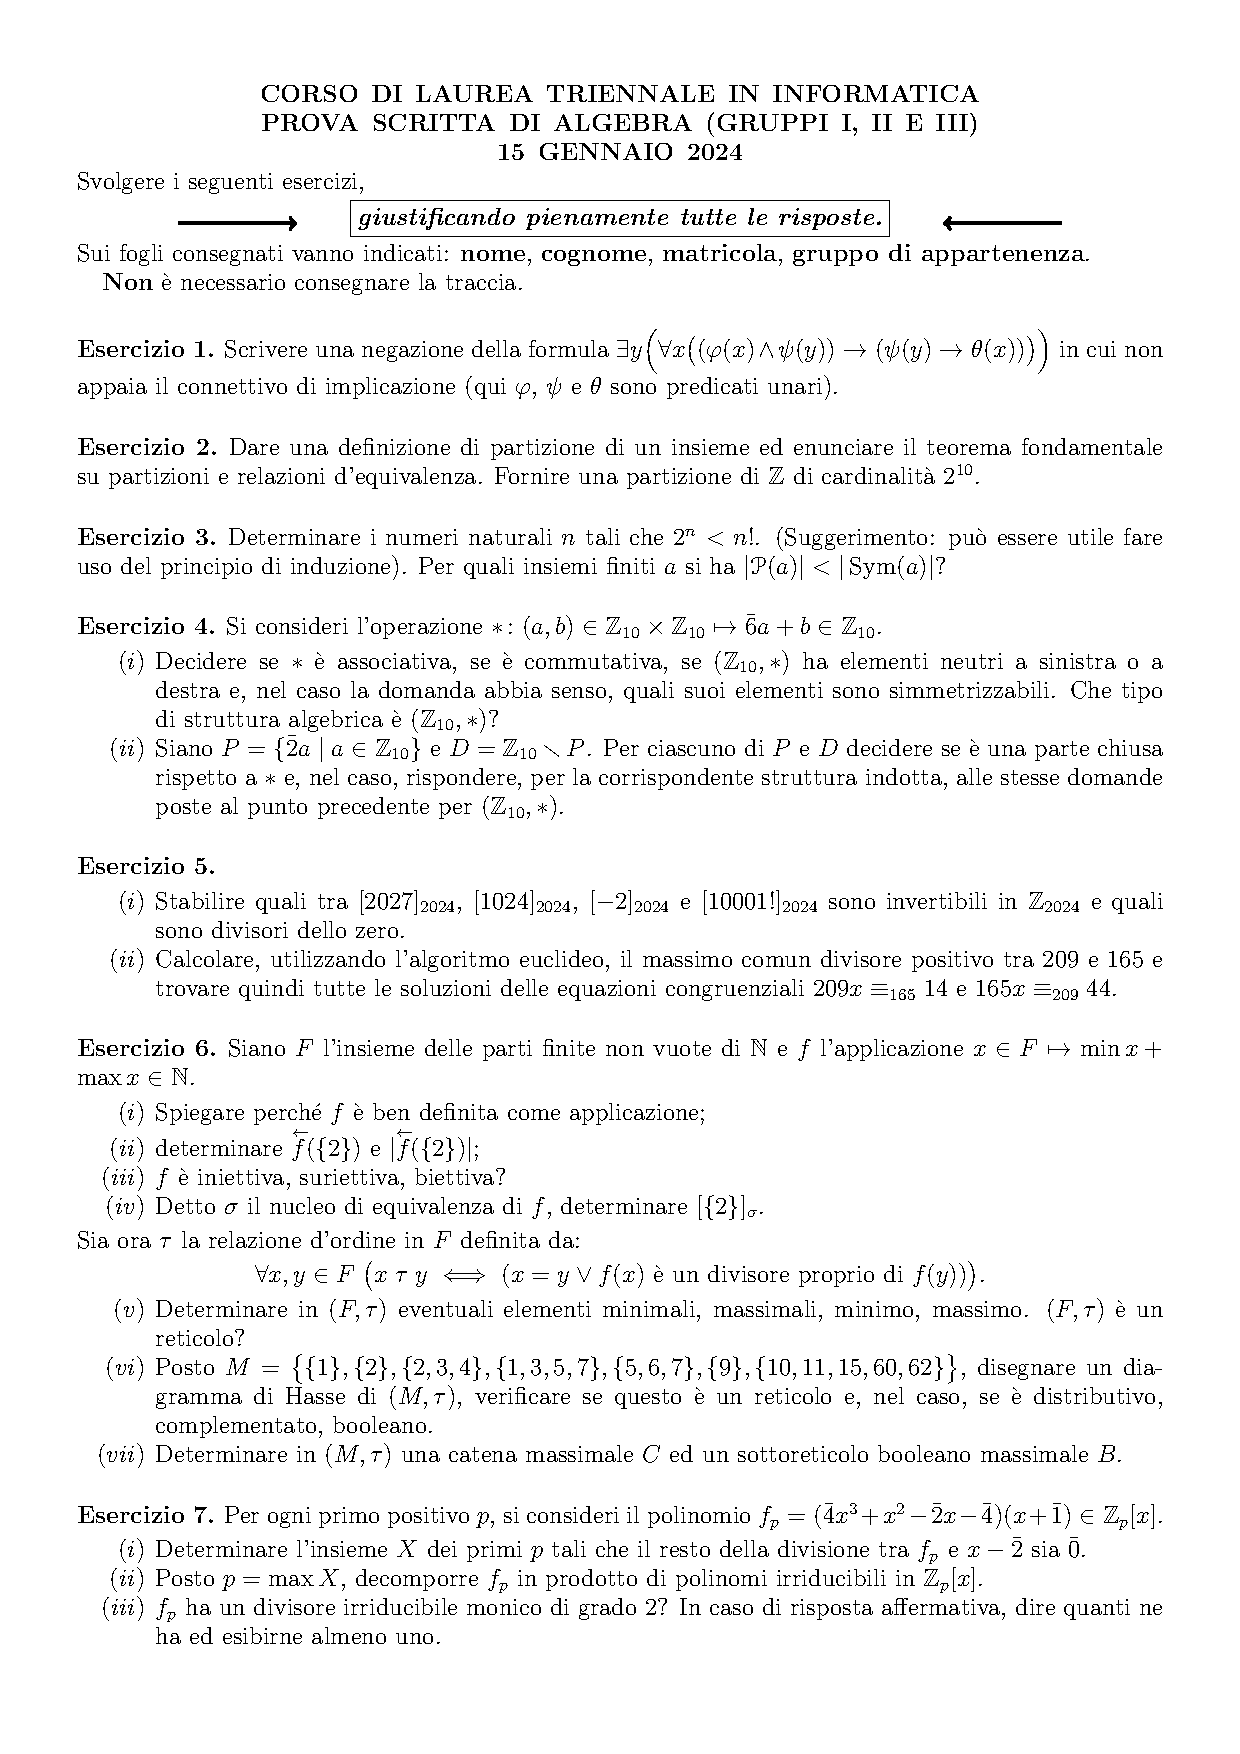
\includegraphics[scale=.85]{pdf/24-01-15}
\end{center}
\subsection*{Esercizio 1}
Applicando la Proposizione \ref{prop:negazione_quantificatori} si ottiene:
\begin{align*}
	\neg \Biggl(\exists y \biggl(\forall x \biggl( \bigl( \varphi(x) \land \psi(y)\bigr)	\implies \bigl(	\psi(y) \implies \theta(x) \bigr)\biggr)\biggr)
	\Biggr) &\iff	\forall y \Biggl(\neg \biggl(\forall x \Bigl( \bigl( \varphi(x) \land \psi(y)		\bigr) \implies \bigl(\psi(y) \implies \theta(x)\bigr)\Bigr) \biggr) \Biggr) \\
	&\iff \forall y 
	\biggl( \exists x \Bigl( \neg  \bigl( \varphi(x) \land \psi(y)\bigr) \implies \bigl(	\psi(y) \implies \theta(x)	\bigr) 	\Bigr)	\biggr) \\
\end{align*}
Poniamo $\alpha \coloneqq \varphi(x) \land \psi(y)$ e $\beta \coloneqq \psi(y) \implies \theta(x)$ e vale, per la Proposizione \ref{prop:negazione_implicazione}:
\begin{align*}
	\neg (\alpha \implies \beta) &\iff \alpha \land \neg (\beta) \\
	&\iff \bigl( \varphi(x) \land \psi(y)\bigr) \land \neg \bigl(\psi(y) \implies \theta(x)\bigr) \\
	&\iff \bigl( \varphi(x) \land \psi(y)\bigr) \land \bigl(\psi(y) \land \neg (\theta(x))\bigr) \\
	&\iff \varphi(x) \land \psi(y) \land \psi(y) \land \neg \bigl(\theta(x)\bigr) \\
	&\iff \varphi(x) \land \psi(y) \land \neg \bigl(\theta(x)\bigr)
\end{align*}
Sostituiamo quindi la formula ottenuta:
\begin{align*}
	\forall y 
	\biggl( \exists x \Bigl( \varphi(x) \land \psi(y) \land \neg \bigl(\theta(x)\bigr)	\Bigr)	\biggr) \\
\end{align*}
\subsection*{Esercizio 2}
Una partizione di un insieme $X$ è un insieme $\mathcal{F}$ di non vuote di $X$ tale insieme, a due a due disgiunte, la cui unione unaria è tutto $X$, ovvero $\bigcup \mathcal{F} = X$. Il Teorema fondamentale su partizioni e relazioni di equivalenza afferma che esiste una corrispondenza biunivoca tra l'insieme delle partizioni di un insieme $A$ e l'insieme delle equivalenze $Eq(A)$, cioè ogni partizione è un insieme quoziente e viceversa. Una partizione di $\mathbb{Z}$ di cardinalità $2^{10}$ è dato dall'insieme quoziente di $\mathbb{Z}$ rispetto alla congruenza modulo $2^{10}$.
\subsection*{Esercizio 3}
Per induzione si dimostra che per ogni $n \geq 4 \bigl( 2^{n} < n! \bigr)$. Infatti:
\begin{itemize}
	\item Se $n=0$ abbiamo $2^{0}=1 = 0!$;
	\item Se $n=1$ abbiamo $2^{1} = 2 > 1 = 1!$;
	\item Se $n=2$ abbiamo $2^{2} = 4 > 2 = 2!$;
	\item Se $n=3$ abbiamo $2^{3} = 8 > 6 = 3!$;
	\item Se $n=4$ abbiamo $2^{4} = 16 < 24 = 4!$;
\end{itemize}
Sia quindi $n>4$ e supponiamo l'asserto vero. Dimostriamo quindi che $2^{n+1}<(n+1)!$. Si ha:
\begin{align*}
	2^{n+1} = 2^{n} \cdot 2
\end{align*}
e 
\begin{align*}
	(n+1)! = (n+1)n!
\end{align*}
Dato che per ipotesi induttiva $2^{n}<n!$ e, dato che $n>4$, sicuramente $2 < n+1$, quindi è lecito eseguire la maggiorazione:
\begin{align*}
	2^{n+1} = 2^{n} \cdot 2 < n! (n+1) = (n+1)!
\end{align*}
Per quanto appena visto possiamo affermare che $|\mathcal{P}(a)| < |Sym(a)|$ per tutti gli insiemi con almeno 4 elementi.
\subsection*{Esercizio 4}
\begin{enumerate}[label=(\textit{\roman*})]
	\item Per ogni terna di elementi $a,b,c \in \mathbb{Z}_{10}$:
	\begin{align*}
		a \ast (b \ast c) &= a \ast (6b +c) \\
		&= 6a +6b+c
	\end{align*}
	e:
	\begin{align*}
		(a \ast b) \ast c &= (6a+b) \ast c \\
		&= 6(6a+b) + c \\
		&= 36a + 6b + c \\
		&= 6a + 6b+c
	\end{align*}
	Quindi $\ast$ è associativa. Siano $a,b \in \mathbb{Z}_{10}$:
	\begin{align*}
		a \ast b = 6a +b \neq  6b +a  = b \ast a
	\end{align*}
	Infatti, presi $a=1$ e $b=0$ abbiamo $a \ast b = 6$ e $b \ast a = 1$. Quindi $\ast$ non è commutativa. Cerchiamo un eventuale neutro a sinistra. Un siffatto elemento, composto a sinistra con qualunque elemento di $\mathbb{Z}_{10}$ deve restituire l'elemento stesso. Ossia:
	\begin{align*}
		\forall x \in \mathbb{Z}_{10} \bigl( t \ast x = x &\iff 6t + x = x  \\
		&\iff 6t = 0 \bigr)
	\end{align*}
	Gli unici $t \in \mathbb{Z}_{10}$ che sono soluzioni di tale equazione risultano essere $t=\overline{5}$ e $t=\overline{0}$. Questi sono gli unici possibili elementi che possono essere neutri a destra. Osserviamo però che, preso un $a \in \mathbb{Z}_{10}$:
	\begin{align*}
		a \ast 0 = 6a  + 0 = a &\iff 5a \equiv_{10} 0 \\ 
		&\iff a = 6 \lor a = 0 
	\end{align*}
	e:
	\begin{align*}
		a \ast 5 = 6a  + 5 = a &\iff 5a \equiv_{10} 5 \\
		&\iff a = \overline{9} \lor a= \overline{1}  \lor a=\overline{3} \lor a = \overline{5} \lor a = \overline{7}
	\end{align*}
	Quindi non risultano essere neutri per tutti gli elementi di $\mathbb{Z}_{10}$.
	\item Abbiamo $P=\{\overline{0},\overline{2},\overline{4},\overline{6},\overline{8}\}$ e $D = \{\overline{1},\overline{3},\overline{5},\overline{7},\overline{9}\}$. Siano $n,m$ due elementi di $\mathbb{Z}_{10}$ e consideriamo i rispettivi elementi $2n$ e $2m$ in P. Allora:
	\begin{align*}
		2n \ast 2m = 12 n + 2m = 2(6n+3m) \in P
	\end{align*}
	Analogamente, un elemento di $D$ è scrivibile come $2n+1$ e abbiamo:
	\begin{align*}
		(2n+1) \ast (2m+1) &= 12n+ 6 + 2m+1  \\
		&= 2(6n+m+3) +1 \in D
	\end{align*}
	Quindi sia $P$ che $D$ sono parti chiuse rispetto a $\ast$. Per le conclusioni del punto precedente $\overline{0}$ non è neutro a destra in $P$ e $\overline{5}$ non è neutro a destra in $D$, quindi $(P,\ast)$ e $(D,\ast)$ sono semigruppi abeliani.
\end{enumerate}
\subsection*{Esercizio 5}
\begin{enumerate}[label=(\textit{\roman*})]
	\item Abbiamo:
	\begin{itemize}
		\item $[2027]_{2024} = [3]_{2024}$. Poiché $(3,2024)=1$ abbiamo che è un elemento invertibile in $\mathbb{Z}_{2024}$;
		\item $[1024]_{2024}$ è un divisore dello zero in quanto è sicuramente non coprimo con $2024$ essendo entrambi numeri divisibili per due.
		\item Analogamente $[-2]_{2024}=[2022]_{2024}$ è un divisore dello zero.
		\item $[10001!]_{2024}=[0]_{2024}$ in quanto $2024$ è uno dei fattori di $10001!$, quindi è un divisore dello zero.
	\end{itemize}
	\item Applicando l'algoritmo delle divisioni successive troviamo:
	\begin{align*}
		209 &= 165 \cdot 1 + 44 \\
		165 &= 44 \cdot 3 + 33 \\
		44 &= 33 \cdot 1 + 11 \\
		33 &= 11 \cdot 3 + 0
	\end{align*}
	Quindi $(209,165)=11$. Dato che $11 \ndivides 14$ possiamo dire che $209x \equiv_{165} 14$ non ammette soluzioni. Al contrario è ovvio che $11 \divides 44$, quindi possiamo trovare delle soluzioni per l'equazione $165 x \equiv_{209} 44$, dividendo tutti i termini per $11$ otteniamo l'equazione congruenziale equivalente:
	\begin{align*}
		15x \equiv_{19} 4
	\end{align*}
	Cerchiamo una combinazione lineare $15x+19y=4$. Mediante l'algoritmo di Euclide abbiamo:
	\begin{align*}
		19 &= 15 \cdot 1 + 4 \\
		15 &= 4 \cdot 3 + 3 \\
		4 &= 3 \cdot 1 + 1 \\
		3 &= 1 \cdot 3 +0 
	\end{align*}
	Quindi $(15,19)=1$. Otteniamo in particolare:
	\begin{align*}
		4 &= 19 + 15\cdot (-1)
	\end{align*}
	Quindi $\overline{-1} = \overline{18}$ è soluzione dell'equazione congruenziale.
\end{enumerate}
\subsection*{Esercizio 6}
\begin{enumerate}[label=(\textit{\roman*})]
	\item Poiché $(\mathbb{N},\leq)$ è un insieme naturalmente ordinato ogni parte finita non vuota di $\mathbb{N}$ risulta dotata di minimo e massimo sicché è possibile sempre eseguire la somma tra questi due valori. Quindi $f$ è ben posta.
	\item Abbiamo:
	\begin{align*}
		\overleftarrow{f}(\{2\}) &= \{x \in F \; | \; f(x) = 2\} \\
		&= \{x \in F \; | \; min(x) + max(x) = 2\} \\
		&= \{ \{0,2\},\{1\},\{0,1,2\}\}
	\end{align*}
	Quindi $|\overleftarrow{f}(\{2\})|=3$.
	\item L'applicazione $f$ non è iniettiva in quanto, per esserlo, dato il Teorema \ref{thm:car_iniettive}, sarebbe dovuto essere $\forall n \in \mathbb{N} \bigl(|\overleftarrow{f}(\{n\})| \leq 1\bigr)$ ma ciò chiaramente non è vero in quanto nel punto precedente è stato trovato un controesempio.
	
	L'applicazione è suriettiva in quanto, per ogni $n \in \mathbb{N}$ è possibile trovare una parte $x \in F$ tale che $min(x)+max(x)=n$. Ad esempio $x=\{1,n-1\}$.
	
	Non essendo iniettiva la funzione non può essere biettiva.
	
	\item Abbiamo:
	\begin{align*}
		[\{2\}]_{\sigma} &= \overleftarrow{f}\bigl(\{f(\{2\})\}\bigr) \\
		&= \overleftarrow{f}(\{4\}) \\
		&= \{\{0,4\},\{0,1,2,3,4\},\{1,2,3\},\{1,3\}\}
	\end{align*}
	
	\item Per le proprietà indotte dalla relazione di divisibilità su $\mathbb{N}$ sappiamo che $\{0,1\} = \overleftarrow{f}(\{1\})$ divide ogni altro $f(y)$ con $y \in F$ risultando quindi il minimo di $(F,\tau)$. Poiché, per ogni $n \in \mathbb{N} \bigl(n \divides 0\bigr)$ abbiamo che $\{0\} \in F$ è il massimo di $(F,\tau)$. La struttura non risulta, però, essere un reticolo in quanto non è possibile determinare, per ogni coppia di elementi inconfrontabili un estremo inferiore ed un estremo superiore in quanto non è possibile determinare un ``massimo comun divisore'' oppure un ''minimo comune multiplo'' tra più parti che condividono la stessa immagine secondo l'applicazione $f$.
	\item Abbiamo:
	\begin{center}
		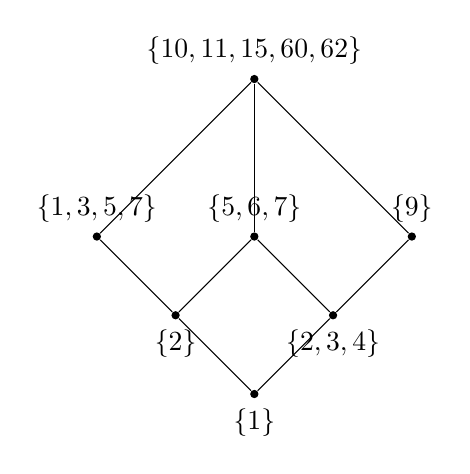
\begin{tikzpicture}
			\node[circle,fill=black,inner sep=0pt,minimum size=3pt,label=below:{$\{1\}$}](a) at (1,0){};
			\node[circle,fill=black,inner sep=0pt,minimum size=3pt,label=below:{$\{2\}$}](b) at (0,1){};
			\node[circle,fill=black,inner sep=0pt,minimum size=3pt,label=below:{$\{2,3,4\}$}](c) at (2,1){};
			\node[circle,fill=black,inner sep=0pt,minimum size=3pt,label=above:{$\{5,6,7\}$}](d) at (1,2){};
			\node[circle,fill=black,inner sep=0pt,minimum size=3pt,label=above:{$\{1,3,5,7\}$}](e) at (-1,2){};
			\node[circle,fill=black,inner sep=0pt,minimum size=3pt,label=above:{$\{9\}$}](f) at (3,2){};
			\node[circle,fill=black,inner sep=0pt,minimum size=3pt,label=above:{$\{10,11,15,60,62\}$}](g) at (1,4){};
			\draw[black,thin](a)--(b);
			\draw[black,thin](a)--(c);
			\draw[black,thin](c)--(f);
			\draw[black,thin](c)--(d);
			\draw[black,thin](b)--(d);
			\draw[black,thin](b)--(e);
			\draw[black,thin](e)--(g);
			\draw[black,thin](d)--(g);
			\draw[black,thin](f)--(g);
		\end{tikzpicture}
	\end{center}
	Chiaramente $(M,\tau)$ è un reticolo ma non è nè distributivo, nè complementato. Infatti è facilmente osservabile il fatto che non esiste alcun complemento per l'elemento $\{5,6,7\}$. Inoltre non è distributivo in quanto il sottoreticolo:
	\begin{center}
		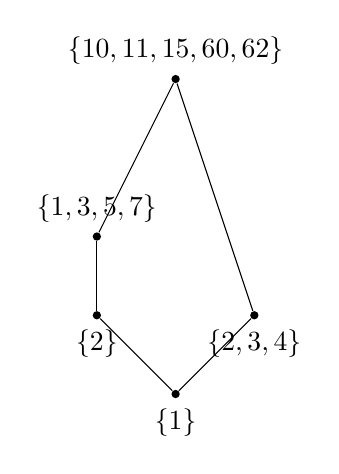
\begin{tikzpicture}
			\node[circle,fill=black,inner sep=0pt,minimum size=3pt,label=below:{$\{1\}$}](a) at (1,0){};
			\node[circle,fill=black,inner sep=0pt,minimum size=3pt,label=below:{$\{2\}$}](b) at (0,1){};
			\node[circle,fill=black,inner sep=0pt,minimum size=3pt,label=below:{$\{2,3,4\}$}](c) at (2,1){};
			
			\node[circle,fill=black,inner sep=0pt,minimum size=3pt,label=above:{$\{1,3,5,7\}$}](e) at (0,2){};
			
			\node[circle,fill=black,inner sep=0pt,minimum size=3pt,label=above:{$\{10,11,15,60,62\}$}](g) at (1,4){};
			\draw[black,thin](a)--(b);
			\draw[black,thin](a)--(c);
			\draw[black,thin](c)--(g);
			\draw[black,thin](b)--(e);
			\draw[black,thin](e)--(g);
		\end{tikzpicture}
	\end{center}
	Risulta essere isomorfo al reticolo pentagonale. Non essendo distributivo chiaramente non può essere booleano.
	\item Una catena massimale $C$ può essere ottenuta dalla parte $\{\{1\},\{2,3,4\},\{9\},\{10,11,15,60,62\}\}$. Un sottoreticolo booleano massimale invece dai quattro elementi: $\{\{1,\{2\},\{2,3,4\},\{5,6,7\}\}\}$.
\end{enumerate}
\subsection*{Esercizio 7} Iniziamo osservando che $\forall p \in \mathbb{P}$ la struttura $(\mathbb{Z}_{p},+,\cdot)$ risulta essere un campo.
\begin{enumerate}[label=(\textit{\roman*})]
	\item Se il resto della divisione tra $f_{p}$ e il polinomio $(x-\overline{2})$ è zero, per il Teorema di Ruffini \ref{thm:ruffini}, $\overline{2}$ è radice di $f_{p}$, cioè $f_{p}(\overline{2})=\overline{0}$. Calcoliamo quindi $f_{p}(\overline{2})$ e calcoliamo per quali $p \in \mathbb{P}$ si annulla:
	\begin{align*}
		(\overline{4}(\overline{2}^{3})+(\overline{2}^{2})-\overline{2}(\overline{2})-4)(\overline{2}+\overline{1}) &= \bigl(\overline{4}\cdot \overline{8} + \overline{4} - \overline{4} - \overline{4}\bigr)\cdot(\overline{3}) \\
		&=\bigl(\overline{32}+\overline{4}-\overline{8}\bigr) \cdot \overline{3} \\
		&=\overline{28} \cdot \overline{3} \\
		&= \overline{84}
	\end{align*}
	Scomponiamo allora $84$ in fattori primi:
	\begin{align*}
		84 = 2^{2} \cdot 7 \cdot 3
	\end{align*}
	Da questa scomposizione possiamo concludere dicendo che, essendo 84 multiplo dei primi 2, 7 e 3, avremo che $\overline{84}=\overline{0}$ in $\mathbb{Z}_{2}, \ \mathbb{Z}_{3}$ e $\mathbb{Z}_{7}$. Quindi $X=\{2,3,7\}$.
	\item Poniamo $p=7=max \ X$. Decomponiamo $f_{7}$ in prodotto di primi irriducibili. Sappiamo che $\overline{2}$ è radice di $f_{7}$, che risulta allora divisibile per $x-\overline{2}$. Notiamo che $f_{7}$ è definito come prodotto tra due polinomi, uno di grado 3 e uno di grado 1. Chiaramente $\overline{2}$ non è radice di $(x+\overline{1})$, per il Lemma \ref{lemma:divisori_prodotto_polinomi} abbiamo quindi che $(x-\overline{2})$ divide $(\overline{4}x^{3}+x^{2}-\overline{2}x-\overline{4})$:
	\begin{center}
		\polylongdiv[style=D]{4x^{3}+x^{2}-2x-4}{x-2}
	\end{center}
	Dove $\overline{28}_{7}=\overline{0}_{7}$ e $\overline{4}x^{2} + \overline{9}x + \overline{16} = \overline{4}x^{2}+\overline{2}x+\overline{2}$. Il polinomio $g_{1}$ così ottenuto risulta essere un polinomio di secondo grado, che sarà irriducibile e solo se non ammette radici. Mediante un controllo diretto si vede facilmente che $g_{1}(\overline{5})=0$. Eseguiamo quindi la divisione di $g_{1}$ per $(x-\overline{5})$:
	\begin{center}
		\polylongdiv[style=D]{4x^{2}+2x+2}{x-5}
	\end{center}
	Con $\overline{112}=\overline{0}$ e $\overline{22}=\overline{1}$. Otteniamo quindi la seguente fattorizzazione:
	\begin{align*}
		f_{7} = (\overline{4}x+\overline{1})(x-\overline{2})(x-\overline{5})(x+\overline{1})
	\end{align*}
	\item Dalla fattorizzazione ottenuta osserviamo che $f_{7}$ non ha alcun divisore monico irriducibile di grado 2.
\end{enumerate}
\vfill
\section{Esame del 16 marzo 2024}
\begin{center}
	\includegraphics[scale=.85]{pdf/24-03-16.pdf}
\end{center}
\subsection*{Esercizio 1}
Poniamo:
\begin{align*}
	\alpha &\coloneqq (p \implies r) \iff(s \lor \neg q) \\
	\beta &\coloneqq (s \land q) \implies (s \lor q)
\end{align*} 
Per verificare allora che $\alpha \implies \beta$ sia una tautologia proviamo che questa non può risultare mai falsa. Per risultare falsa deve essere vera $\alpha$ e falsa $\beta$. Se $\beta$ risultasse falsa avremmo che $(s \land q)$ debba risultare vera mentre $(s \lor q)$ falsa. Però, se $(s \land q)$ è vera, lo saranno sia $s$ che $q$, quindi $(s \lor q)$ in particolare non potrebbe risultare falsa. Da questo controsenso possiamo concludere che $\alpha \implies \beta$ è una tautologia. \hfill \blacksquare
\subsection*{Esercizio 2}
\begin{enumerate}[label=(\textit{\roman*})]
	\item La funzione non è iniettiva. Infatti prese le coppie $(1,0)$ e $(-1,60)$ otteniamo:
	\begin{displaymath}
		f((1,0)) = 30 \cdot 1 + 0 = 30 = 30 \cdot -1 + 60 = f((-1,60))
	\end{displaymath}
	\item La funzione è suriettiva, infatti per ogni $z \in \mathbb{Z}$ abbiamo che $z = f(0,z)$. Quindi, per ogni numero intero $z \in \mathbb{Z}$ esiste una coppia $(a,b) \in \mathbb{Z} \times \mathbb{Z}$ tale che $f((a,b))=z$.
	\item Un elemento $[f(a,b)]_{45} \in \mathbb{Z}_{45}$ risulta essere invertibile se e solo se $MCD(f(a,b),45)=1$. Ovvero se non esiste alcun divisore comune diverso da 1 tra di loro.
	
	Per avere che un numero intero della forma $30a+b$ sia coprimo con 45 sarà necessario assicurarsi che questo non condivida alcun fattore primo con $45$, cioè non essere divisibile né per 3 né per 5, in quanto $45=3^{2}\cdot 5$. Essendo $30=3 \cdot 5 \cdot 2$, un intero della forma $30a$ avrà sempre divisori in comune con $45$, quindi sarà sufficiente imporre a $b$ di non annullare i contributi di $3$ e $5$ in $a$. Ovvero imponendo che $b$ non sia divisibile per $3$ e $5$.
	
	Possiamo quindi descrivere $S$ come l'insieme delle coppie $(a,b)$ con $a \in \mathbb{N}$ e $b \in \{61,62,64,67,68\}$.
	\item Presa la coppia $(0,61)$ procediamo a calcolare l'inverso di $[61]_{45}=[16]_{45}$. Cerchiamo dunque un elemento $x \in \mathbb{Z}_{45}$ tale che $16x \equiv_{45} 1$. Procediamo utilizzando l'algoritmo delle divisioni successive:
	\begin{align*}
		45 &= 16 \cdot 2 + 13 \\
		16 &= 13 \cdot 1 + 3 \\
		13 &= 3 \cdot 4 + 1 \\
		3 &= 1 \cdot 3 + 0
	\end{align*}
Si ottiene quindi:
\begin{align*}
	1 &= 13 +(-4)3 \\
	&= (45 +(-2)16) + (-4)(16+(-1)13) \\
	&= 45 + (-6)16 +(4)45 + (-8)16 \\
	&= (5)45+(-14)16
\end{align*}
Da cui possiamo vedere che $x=[-14]_{45}=[31]_{45}$ è la soluzione cercata. 

\end{enumerate}
\subsection*{Esercizio 3}
\begin{enumerate}[label=(\textit{\roman*})]
	\item $|R| = |\mathbb{Z}_{4}| \times |\mathbb{Z}_{6}| = 4 \cdot 6 = 24$.
	\item Si ha $0_{R}=(0,0)$ e $1_{R}=(1,1)$. Infatti, per ogni coppia $(a,b) \in R$ si ha:
	\begin{align*}
		(a,b)+(0,0) =(a+0,b+0)=(a,b) \\
		(a,b)\cdot(1,1)=(1\cdot a, 1 \cdot b) = (a,b)
	\end{align*}
	Un elemento $(a,b) \in R$ è invertibile se esiste un elemento $(a',b')$ tale che:
	\begin{displaymath}
		(a,b) \cdot (a',b') = (a \cdot a', b \cdot b') = (1,1)
	\end{displaymath}
	La ricerca di tali coppie in $R$ può essere ridotta quindi alla ricerca degli elementi invertibili in $\mathbb{Z}_{4}$ e $\mathbb{Z}_{6}$. Per la Proposizione \ref{prop:invertibili_zm} sappiamo che in $\mathbb{Z}_{4}$ risultano essere invertibili gli elementi $\overline{1}$ e $\overline{3}$ mentre in $\mathbb{Z}_{6}$ sono invertibili gli elementi $\overline{5}$ e $\overline{1}$. Otteniamo così le seguenti 4 coppie di elementi invertibili:
	\begin{displaymath}
		\mathcal{U}(R,\cdot) =\{(1,1),(1,5),(3,1),(3,5)\}
	\end{displaymath}
	Facendo un ragionamento analogo otteniamo che in $\mathbb{Z}_{4}$ risultano essere divisori dello zero gli elementi $\overline{0}$ e $\overline{2}$ mentre sono divisori dello zero in $\mathbb{Z}_{6}$ gli elementi $\overline{0},\ \overline{2}, \ \overline{3}, \ \overline{4}$. Le coppie di $R$ che risultano essere divisori dello zero sono quindi:
	\begin{displaymath}
		\{(0,0),(0,2),(0,3),(0,4),(2,0),(2,2),(2,3),(2,4)\}
	\end{displaymath}
	Un elemento $(a,b) \in R$ è idempotente se, e soltanto se, $(a,b) \cdot (a,b) = (a,b)$. In altre parole deve essere:
	\begin{displaymath}
		\begin{cases}
			a^{2} \equiv_{4} a \\
			b^{2} \equiv_{6} b
		\end{cases}
	\end{displaymath}
	L'equazione $a^{2} \equiv a (mod 4)$ è equivalente all'equazione $a^{2} \equiv a (mod 2)$ che è sua volta equivalente a $a(a-1) \equiv 0 (mod 2)$ che ha soluzioni solo per $a=0, \ a= 1$ per la legge di annullamento del prodotto. Seguendo un ragionamento analogo, l'equazione $b^{2}\equiv b (mod 6)$ è risolta da $b \in \{0,1,3,4\}$. Otteniamo quindi che le coppie:$$(0,0), \ (0,1),\ (0,3),\ (0,4),\ (1,0),\ (1,1),\ (1,3), \ (1,4)$$ risultano essere idempotenti in $R$.
	\item Un elemento di $R$ è radice del polinomio $x^{2}-x$ se e soltanto se:
	\begin{align*}
		(a,b)\cdot (a,b) - (a,b) = (0,0) &\iff (a^{2}-a,b^{b}-b) = (0,0) \\
		&\iff \begin{cases*}
			a^{2} = a \\
			b^{2} = b
		\end{cases*}
	\end{align*}
Quindi tutte le coppie di elementi idempotenti in $R$ trovate nel punto precedente sono radici di tale polinomio.
	\item Risulta $mcm(4,6)=12$ e vale $12 \cdot 1_{R}=12 \cdot (1,1)=(12,12)=(0,0)=0_{R}$, quindi la caratteristica di $R$ è 12.
	\item $R$ non è un dominio di integrità in quanto sono presenti divisori dello zero.
	\item Siano $(a,b),(c,d) \in M$ e consideriamo le composte $(a,b)+(c,d) =(a+c,b+d)$ e $(a,b)\cdot(c,d)=(ac,bd)$. Per verificare la stabilità di $M$ deve essere $b+d \in \{[0]_{6},[3]_{6}\}$ e $bd \in \{[0]_{6},[3]_{6}\}$, che risulta banalmente vero. $(M,+,\cdot)$ risulta quindi essere un anello commutativo. 
	\item $(M,+,\cdot)$ è un anello unitario in quanto la coppia $(1,3) \in M$ risulta essere un elemento neutro rispetto alla moltiplicazione, quindi $(M,\cdot)$ è un monoide.
\end{enumerate}
\subsection*{Esercizio 4}
La relazione $\rho$ è una relazione d'ordine. Infatti:
\begin{itemize}
	\item È \textit{riflessiva}: $\forall a \in \mathbb{N} \bigl( a \ \rho \ a \iff (a-a)=0=2a\cdot 0 \in 2a\mathbb{N}\bigr)$;
	\item È \textit{antisimmetrica}: siano $a,b \in \mathbb{N}$ tali che $a \ \rho \ b$ e $b \ \rho \ b$. Allora vale, per opportuni $k,m \in \mathbb{N}$:
	\begin{align*}
		\begin{cases}
			b-a &= 2ak \\
		a-b &= 2bm
		\end{cases}
	\implies 
	\begin{cases}
		b = 2ak+a = a(2k+1)\\
		a = 2bm+b = b(2m+1)
	\end{cases}
	\end{align*}
Sostituendo la seconda equazione nella prima si ottiene:
\begin{align*}
	a = \bigl(a (2m+1)(2k+1)\bigr)
\end{align*}
Per cui deve essere $(2m+1)(2k+1)=1$ che risulta vera se e solo se $m=k=0$, allora sostituendo tali valori nelle prime equazioni si ottiene $b-a=0 \iff b=a$.
\item È \textit{transitiva:} siano $a,b,c \in \mathbb{N}$ tali che $a \ \rho \ b$ e $b \ \rho \ c$. Quindi $b-a \in 2a\mathbb{N}$ e $c-b \in 2b\mathbb{N}$. Dimostriamo che $c-a \in 2a\mathbb{N}$. Ripetendo un ragionamento analogo a quanto visto per dimostrare l'antisimmetria della relazione $\rho$, abbiamo che $b = a(2k+1)$ e $c=b(2m+1)$ per un opportuni $k,m \in \mathbb{N}$. Sostituendo l'equazione di $b$ nella seconda si ottiene:
\begin{align*}
	c&=b(2m+1) \\
	&=\bigl(a(2k+1)\bigr)(2m+1)
\end{align*}
Calcoliamo quindi la differenza $c-a$:
\begin{align*}
	c-a &= \bigl(a(2k+1)\bigr)(2m+1) -a \\
	&= a \bigl((2k+1)(2m+1)-1\bigr) \\
	&= a \bigl(4km + 2k +2m + 1 -1\bigr) \\
	&= a \bigl(2(km+k+m)\bigr) \\
	&= a \cdot 2 \nu \in 2a \mathbb{N} & \text{\textcolor{gray}{(Ponendo $km+k+m = \nu $)}}
\end{align*}
Il che dimostra la transitività della relazione $\rho$.
\end{itemize}
\begin{enumerate}[label=(\textit{\roman*})]
	\item L'insieme dei minoranti di $\{12\}$ è definito come:
	\begin{displaymath}
		\{12\}^{\downarrow} = \{ n \in \mathbb{N} \; | \; n \ \rho \ 12 \}
	\end{displaymath}
	Un naturale $n \in \mathbb{N}$ ``precede'' $12$ se e solo se:
	\begin{align*}
		n \ \rho \ 12 &\iff 12 -n  \in 2n\mathbb{N} \\
		&\iff \exists k \in \mathbb{N} \bigl(12 -n = 2nk\bigr)\\
		&\iff \exists k \in \mathbb{N} \bigl(12 = n +2nk\bigr)\\
		&\iff \exists k \in \mathbb{N} \bigl(12 = n(2k+1)\bigr)\\
	\end{align*}
Quindi se, e solo se $n \divides 12$ e $12/n$ è dispari. I divisori di 12 sono $\{1,2,3,4,6,12\}$, eseguendo dei rapidi calcoli otteniamo che per $n=4$ si ottiene $12/4=3$ e per $n=12$ si ha $12/12=1$. Quindi:
\begin{displaymath}
	\{12\}^{\downarrow} = \{4,12\}
\end{displaymath}
\item Un elemento $a \in \mathbb{N}$ è minimale se e solo se non esiste un naturale $b \in \mathbb{N}$ tale che sia $b \neq a$ e $b \ \rho \ a$. Ossia:
\begin{align*}
	a \ \text{minimale in $\mathbb{N}$} &\iff \neg \bigl(\exists b \in \mathbb{N}( b \ \rho \ a \land b \neq a)\bigr) \\
	&\iff \neg \bigl(\exists b \in \mathbb{N}( a-b \in 2b\mathbb{N} \land b \neq a)\bigr) \\ 
	&\iff \neg \bigl(\exists b \in \mathbb{N}( b \divides a \land \exists k \in \mathbb{N}(\frac{a}{b} = (2k+1)) \land b \neq a)\bigr) \\
\end{align*}
Chiaramente $1$ risulta minimale in $\mathbb{N}$, così come il 2. Ogni numero dispari è preceduto da almeno $1$ e non può appartenere quindi all'insieme dei minimali. Infatti, preso un numero dispari della forma $m= (2k+1)$ abbiamo che $1 \divides m$ e $\frac{m}{1} = 2k+1$. Restano da analizzare quindi solo i numeri pari, ovvero gli elementi dell'insieme $2\mathbb{N}=\{2t \; | \; t \in \mathbb{N} \}$. Se $t$ è dispari abbiamo che il numero $n = 2t$ può essere scritto come $2 \cdot (2k+1)$ ed è chiaro che $(2k+1) \ \rho \ n$. Sia $t$ pari, in questo caso $n$ risulta essere una potenza del 2 che può essere scritta come $2^{k}$. Gli unici divisori propri di $2^{k}$ saranno le potenze del tipo $2^{j}$ con $j < k$ e $\frac{2^{k}}{2^{j}}=2^{k-j}$ che risulta essere pari. Possiamo affermare quindi che, se $n$ è una potenza del due, non esistono naturali $m$, diversi da $n$ stesso, che dividano $n$ e tali che $\frac{n}{m}$ sia dispari. Quindi l'insieme elementi minimali di $(\mathbb{N},\rho)$ è rappresentato da tutte le potenze del 2. Avendo infiniti minimali non esiste il minimo in $(\mathbb{N},\rho)$. 

Dato che ogni numero è ``coperto'' da un suo multiplo, non esistono elementi massimali in $\mathbb{N}$, e di conseguenza neanche massimi.
\item Considerata una qualsiasi coppia di elementi $\{2^{i},2^{j}\}$ con $i,j \in \mathbb{N}$ osserviamo che non esiste estremo inferiore in $(\mathbb{N},\rho)$ il quale non risulta essere quindi un reticolo.
\item Sia $f: (\mathbb{N},\rho) \rightarrow (\mathbb{N},\divides)$ l'applicazione identica. Chiaramente questa risulta crescente per come è definita la relazione $\rho$. Infatti, presi $a, b \in \mathbb{N}$:
\begin{align*}
	a \ \rho \ b &\iff b-a \in 2a\mathbb{N} \\
	&\iff \exists k \in \mathbb{N} \bigl( b= 2ak+a\bigr) \\
	&\iff \exists k \in \mathbb{N} \bigl(b=a(2k+1)\bigr) \\
	&\iff a \divides b\\
	&\iff f(a) \divides f(b)
\end{align*}
L'applicazione identica è biettiva, crescente, ma non lo è l'applicazione inversa $f^{-1}$. Infatti, presi due elementi $a,b \in \mathbb{N}$ tali che $a \divides b$, non è detto che $b$ sia esprimibile necessariamente come prodotto di $a$ per un numero dispari, condizione necessaria affinché $a \ \rho \ b$. Ad esempio presa la coppia $(4,8)$ vale $4 \divides 8$ eppure $ 4 \ \cancel{\rho} \ 8$ in quanto $8-4 \notin 2 \cdot 4 \mathbb{N} = 8\mathbb{N}$. Quindi $f$ non risulta essere un isomorfismo.
\item Si ha:
\begin{center}
	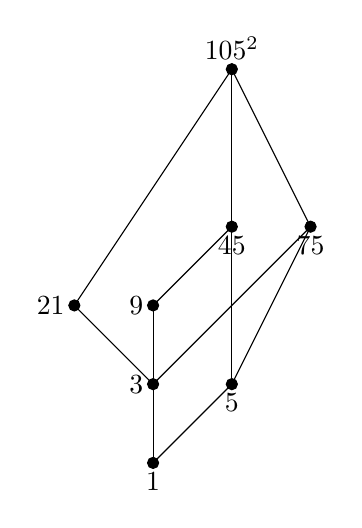
\begin{tikzpicture}
		\filldraw[black] (0,0) circle(2pt) node[anchor=north]{1};
		\filldraw[black] (0,1) circle(2pt) node[anchor=east]{3};
		\filldraw[black] (1,1) circle(2pt) node[anchor=north]{5};
		\filldraw[black] (0,2) circle(2pt) node[anchor=east]{9};
		\filldraw[black] (-1,2) circle(2pt) node[anchor=east]{21};
		\filldraw[black] (1,3) circle(2pt) node[anchor=north]{45};
		\filldraw[black] (2,3) circle(2pt) node[anchor=north]{75};
		\filldraw[black] (1,5) circle(2pt) node[anchor=south]{$105^{2}$};
		\draw[black](0,0)--(0,1);
		\draw[black](0,0)--(1,1);
		\draw[black](0,1)--(0,2);
		\draw[black](0,1)--(2,3);
		\draw[black](0,2)--(1,3);
		\draw[black](0,1)--(-1,2);
		\draw[black](-1,2)--(1,5);
		\draw[black](1,3)--(1,5);
		\draw[black](1,1)--(1,3);
		\draw[black](1,1)--(2,3);
		\draw[black](2,3)--(1,5);
	\end{tikzpicture}
\end{center}
$(S,\rho)$ è un reticolo.
\end{enumerate}
\subsection*{Esercizio 5}
Una relazione binaria è una terna $\rho = (A,A,G)$ dove $A$ è un insieme e $G\subseteq A\times A$.
\begin{enumerate}[label=(\textit{\roman*})]
	\item Preso $a=\{1,2,3,4,5,6,7\}$ consideriamo tutte le relazioni $\sim=(A,A,G)$ dove:
	\begin{align*}
		\{(0,7),(1,4),(2,3),(2,4),(2,7)\} \subseteq G
	\end{align*}
	Inoltre, se la coppia $(3,1)$ appartiene al grafico allora anche la coppia $(5,0) \in G$. Per la proprietà transitiva sappiamo che $(1 \sim 4) \land (4  \sim  2)$, quindi $(1,2) \in G$. Analogamente, da $(0  \sim  7) \land (7 \sim 2)\implies (0 \sim 2)$. Infine, essendo $(3 \sim  2) \land (2 \sim 0) \implies (3 \sim 0) \implies (5 \sim 0)$. La parte $[2]_{\sim}=\{0,1,2,3,4,5,7\}$ risulta quindi un'unica classe di equivalenza, dalla quale resta escluso l'elemento 6. Possiamo considerare quindi due casi, e di conseguenza due relazioni di equivalenza: 
	\begin{enumerate}
		\item Se 6 è in relazione con un elemento di $[2]_{\sim}$ allora $\sim_{1} = \tau_{A}$ è la relazione totale.
		\item Se 6 non è in relazione con alcun elemento di $[2]_{\sim}$ allora sarà in relazione $\sim_{2}$ solo con sè stesso.
	\end{enumerate}
	
	\item Per il Teorema \ref{thm:equivalenza_partizione} esiste una applicazione biunivoca tra l'insieme $Eq(a)$ e $Partz(a)$. Si ottengono le due partizioni:
	\begin{itemize}
		\item $A/\{\sim_{1}\}=A/\{\tau_{A}\}=\{A\}$
		\item $A/{\sim_{2}}=\{[2]_{\sim},[6]_{\sim}\}$ dove $[6]_{\sim}=\{6\}$.
	\end{itemize}
\end{enumerate}
\begin{center}
	\begin{tikzpicture}[scale=1.5]
		
		% Coordinate for the elements
		\coordinate (A1) at (0, 0);
		\coordinate (A2) at (1, 0);
		\coordinate (A3) at (2, 0);
		\coordinate (A4) at (3, 0);
		\coordinate (A5) at (1, 1);
		\coordinate (A6) at (2, 2);
		\coordinate (A7) at (3, 1);
		
		% Draw elements
		\foreach \i/\j in {1/A1, 2/A2, 3/A3, 4/A4, 5/A5, 6/A6, 7/A7} {
			\draw[fill=white] (\j) circle [radius=0.2];
			\node at (\j) {\i};
		}
		
		% Highlight the subset {1,2,3,4,5,7}
		\draw[rounded corners=8pt, thick, dashed, red] 
		($(A1)+(-0.4,-0.4)$) rectangle ($(A7)+(0.4,0.4)$);
		\node[shape=circle,draw=blue, minimum width=1.5cm, dashed, fit={(A6)}]{};
		\node[shape=circle,draw,minimum width=8cm,fit={(A1)(A2)(A3)(A4)(A5)(A6)}]{};
	\end{tikzpicture}
	\captionof{figure}{Partizione determinata dalla relazione $\sim_{2}$}\label{fig:15324_4}
\end{center}
\subsection*{Esercizio 6}
Partiamo con l'osservare che $(\mathbb{Z}_{11}[x])$ è un campo. Il polinomio $(x^{2}-5)$ può essere scritto come:
\begin{align*}
	(x^{2}-5) = (x+4)(x-4) = (x-7)(x+7)
\end{align*} 
In quanto $4^{2} = \overline{16}_{11} = \overline{5}_{11}$ e anche $\overline{7}^{2} = \overline{49}_{11} = \overline{5}_{11}$.
Procediamo ora a calcolare $g(1)$ e $g(-1)$:
\begin{align*}
	g(1)&=(\overline{1})^{5}+4(\overline{1})^{2}-\overline{1}+\overline{7}=\overline{11}=\overline{0} \\
	g(-1) &= (\overline{-1})^{5} + 4(\overline{-1})^{2} + \overline{1} +\overline{7} = \overline{11} = 0
\end{align*}
Quindi $(x-1) \divides_{\mathbb{Z}_{11}} g$ e $(x+1) \divides_{\mathbb{Z}_{11}} g$. Procediamo quindi a fattorizzare il polinomio $g$ eseguendo la divisione lunga:
\begin{center}
	\polylongdiv[style=D]{x^{5}+4x^{2}-x+7}{x-1}
\end{center}
Dato che $\overline{11}=\overline{0}$ abbiamo ottenuto un divisore $g_{1}=x^{4}+x^{3}+x^{2}+5x+4$ che sarà divisibile per $x=-1$. Infatti, essendo $g(x) =g_{1} \cdot (x-1)$, deve valere:
\begin{align*}
	g(-1) &= g_{1}(-1) \cdot (-1 - 1) \\
	&= g_{1}(-1) \cdot (-2) = \overline{0}	\\
	&\iff g_{1}(-1) = 0 \\
	&\iff (x+1) \divides_{\mathbb{Z}_{11}} g_{1}
\end{align*}
Possiamo quindi eseguire la divisione:
\begin{center}
	\polylongdiv[style=D]{x^{4}+x^{3}+x^{2}+5x+4}{x+1}
\end{center}
Verifichiamo che $g_{3}$ sia irriducibile. Se non lo fosse dovrebbe esistere una $x \in \mathbb{Z}_{11}$ tale che $x^{3}+x+4\equiv_{11} 0$, in particolare deve essere $x^{3}+x=7$, il quale sommato a $4$, annullerebbe il polinomio. Dato che non esiste un intero $n \in \mathbb{Z}$ tale che $n^{3}+n \equiv_{11} 7$, abbiamo che $g_{2} = x^{3}+x+4$ è irriducibile. Otteniamo quindi la fattorizzazione:
\begin{align*}
	f = (x+4)(x-4)(x^{3}+x+4)(x+1)(x-1)
\end{align*}
\begin{enumerate}[label=(\textit{\roman*})]
	\item Il polinomio $f$ non è esprimibile come prodotto di sei polinomi non costanti.
	\item Il polinomio $f$ non è esprimibile come prodotto di polinomi irriducibili non monici con tutti lo stesso coefficiente direttore in quanto qualsiasi coefficiente $a \neq 1$, moltiplicato ai fattori di $f$, restituirebbe un polinomio $a \cdot f$ diverso da $f$ stesso.
\end{enumerate}
\vfill

\section{Esame del 22 aprile 2024}
\begin{center}
	\includegraphics[scale=.85]{pdf/24-04-22.pdf}
\end{center}
\subsection*{Esercizio 1}
\begin{enumerate}[label=(\textit{\roman*})]
	\item Il Teorema fondamentale su partizioni e relazioni di equivalenza afferma che esiste una corrispondenza biunivoca tra l'insieme delle partizioni di un insieme $A$ e l'insieme delle equivalenze $Eq(A)$, cioè ogni partizione è un insieme quoziente e viceversa.
	\item Un insieme $\mathcal{F}$ per essere una partizione con due elementi deve essere costituita da due parti disgiunte di $T$, $F_{3}$ e $F_{2}$, tali che $|F_{1}|=3$ e $|F_{2}|=2$, oppure da $F_{1}$ ed $F_{4}$ con $|F_{1}|=1$ ed $|F_{4}|=4$. Il numero di parti di $T$ con tre elementi è dato da:
	\begin{align*}
		\binom{5}{3} = \frac{5!}{3!2!} = 10
	\end{align*}
Fissati tre elementi di $T$ a costituire una parte restano solo due elementi ``liberi'' per poter costituire $F_{2}$, esistono quindi $10 \cdot 1$ possibili combinazioni tra $F_{2}$ ed $F_{3}$ per costruire una partizione di $T$ con cardinalità 2. Il numero di parti con 4 elementi è invece dato da:
\begin{align*}
	\binom{5}{4} = \frac{5!}{4!}= 5
\end{align*}
Fissati quattro elementi di $T$ a costituire una parte $F_{4}$ resta una sola opzione per costruire una parte di un singolo elemento. Quindi il numero totale di partizioni di cardinalità 2 è 15.
\item Abbiamo:
\begin{itemize}
	\item $1+3=4$
	\item $2+4=6$
	\item $2+0+2=4$
	\item $1+1+0+4=6$
	\item $1+1+0+2+1+1=6$
\end{itemize}
Quindi $T/{\alpha}=\{\{13,202\},\{24,1104,110211\}\}$.
	\end{enumerate}
\subsection*{Esercizio 2}
\begin{enumerate}[label=(\textit{\roman*})]
\item Si ha: 
\begin{itemize}
	\item $\overrightarrow{f}(\mathbb{N} \times \mathbb{N}^{*})=\mathbb{N}$
	\item $\overrightarrow{f}(\emptyset) = \emptyset$
	\item $\overleftarrow{f}(\emptyset) = \emptyset$
	\item $\overleftarrow{f}(\{1\})=\{(1,n) \; | \; n \in \mathbb{N}^{*}\}$
	\item $\overleftarrow{f}(\{5\})=\{(5,1)\}$
\end{itemize}
\item L'applicazione $f$ non è iniettiva in quanto $f((0,1))=f((0,2))=0$ ma $(0,2) \neq (0,1)$. La funzione è suriettiva in quanto per ogni $n \in \mathbb{N}$ possiamo individuare una coppia $(a,b) \in \mathbb{N} \times \mathbb{N}^{*}$ tale che $f((a,b))=n$, infatti $f((n,1))=n^{1}=n$. L'applicazione, non essendo iniettiva, non è biettiva.
\item Un insieme ordinato $(S,\leq)$ è un reticolo se, e soltanto se, per ogni parte $\{a,b\} \subseteq S$ esiste estremo inferiore ed estremo superiore.
\item Il minimo di $(\mathbb{N}\times \mathbb{N}^{*})$ è dato dalla coppia $(1,1)$ in quanto, in $\mathbb{N}$, $f((1,1))=1$ divide ogni altro naturale. Poiché non esiste alcuna coppia la cui immagine secondo $f$ sia nulla, non esiste massimo e, avendo escluso tale valore, non esistono valori massimali in quanto ogni naturale non nullo è divisore dei suoi multipli. La struttura $(\mathbb{N}\times \mathbb{N}^{*},\tau)$ non è un reticolo in quanto, prese ad esempio le coppie $\bigl\{(1,2),(2,1)\bigr\}$, abbiamo:
\begin{align*}
	\bigl\{(1,2),(2,1)\bigr\}^{\uparrow} = \{(2,2),(4,1)\}
\end{align*}
e non esiste un minimo di tale insieme, ossia non esiste un estremo superiore.
\item Essendo:
\begin{itemize}
	\item $f((4,1))=4^{1}=4$
	\item $f((2,2))=2^{2}=4$
	\item $f((2,3))=2^{3}=8$
	\item $f((6,2))=6^{2}=36$
	\item $f((4,2))=4^{2}=16$
	\item $f((12,2))=12^{2}=144$
\end{itemize} 
Abbiamo:
\begin{center}
	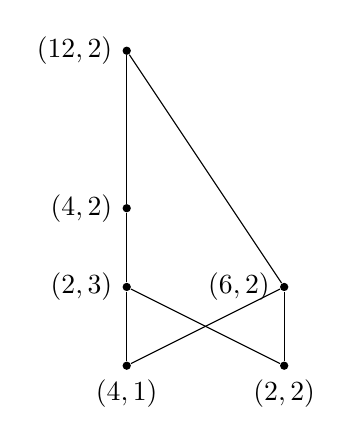
\begin{tikzpicture}
		\node[circle,fill=black,inner sep=0pt,minimum size=3pt,label=below:{$(4,1)$}](a) at (0,0){};
		\node[circle,fill=black,inner sep=0pt,minimum size=3pt,label=below:{$(2,2)$}](b) at (2,0){};
		\node[circle,fill=black,inner sep=0pt,minimum size=3pt,label=left:{$(2,3)$}](c) at (0,1){};
		\node[circle,fill=black,inner sep=0pt,minimum size=3pt,label=left:{$(6,2)$}](d) at (2,1){};
		\node[circle,fill=black,inner sep=0pt,minimum size=3pt,label=left:{$(4,2)$}](e) at (0,2){};
		\node[circle,fill=black,inner sep=0pt,minimum size=3pt,label=left:{$(12,2)$}](f) at (0,4){};
		\draw[black,thin] (a)--(c);
		\draw[black,thin] (b)--(c);
		\draw[black,thin] (a)--(d);
		\draw[black,thin] (b)--(d);
		\draw[black,thin] (c)--(e);
		\draw[black,thin] (d)--(f);
		\draw[black,thin] (e)--(f);
	\end{tikzpicture}
\end{center}
\item $(M,\tau)$ non è un reticolo in quanto non esiste un minimo. Eliminando la coppia $(2,2)$ otteniamo un reticolo distributivo, complementato, e quindi booleano.
\end{enumerate}

\subsection*{Esercizio 3}
\begin{enumerate}[label=(\textit{\roman*})]
	\item Un semigruppo è una struttura $(S,\bot)$ in cui $\bot$ è associativa. $(\mathbb{Z}_{6},\ast)$ è un semigruppo in quanto, per ogni terna di elementi $a,b,c \in \mathbb{Z}_{6}$ abbiamo:
	\begin{align*}
		a \ast (b \ast c) &= a \ast (3b + 4c ) \\
		&= 3a + 4(3b+4c) \\
		&= 3a + 12b + 16c \\
		&= 3a + 4c
	\end{align*}
e:
\begin{align*}
	(a \ast b) \ast c &= (3a+4b) \ast c \\
	&= 3(3a+4b)+4c \\
	&= 9a + 12b + 4c \\
	&= 3a + 4c
\end{align*}
\item L'operazione non è commutativa, presi $a=1$ e $b=0$ si ha ad esempio $a \ast b = 1 \neq 4 = b \ast a$.
\item Si ha: $0 \ast 0 = 0$, $0 \ast 3 = \overline{12}=\overline{0}$, $3 \ast 0 = \overline{9}=\overline{3}$, $3 \ast 3 = 3$. Quindi $\{0,3\}$ è stabile.
\end{enumerate}
\subsection*{Esercizio 4}
\begin{enumerate}
	\item Essendo $\rho$ una relazione binaria antiriflessiva e simmetrica la coppia $(\mathbb{Z},\rho)$ risulta essere un grafo.
	\item Un albero è un grafo connesso senza circuiti. Consideriamo l'insieme $S=\{1,2,4,10,20\}$ e l'insieme dei lati:
	\begin{align*}
		L = \{(1,2),(1,4),(1,10),(1,20)\}
	\end{align*}
Si ottiene così il seguente albero:
\begin{center}
	\begin{forest}
	for tree={circle,draw}
		[1
			[2]
			[4]
			[10]
			[20]
		]
	\end{forest}
\end{center}
\end{enumerate}

\subsection*{Esercizio 5}
\begin{enumerate}[label=(\textit{\roman*})]
	\item Siano $\overline{3}$ e $\overline{5}$ radici di $f$. Ciò significa che, per il teorema di Ruffini generalizzato, $(x-3)(x-5)$ divide $f$. Sviluppando $(x-3)(x-5)$ otteniamo il polinomio $(x^{2}-8x+2)$, quindi $f$ è un multiplo di $(x^{2}-8x+2)$. Analogamente, se $f$ è un multiplo di $(x^{2}-8x+2)$, essendo $\mathbb{Z}_{13}$, le sue radici sono tutte e sole le radici dei suoi multipli. Quindi l'equivalenza è vera.
	\item Il polinomio $(x^{2}-8x+2)$ non è irriducibile in quanto ammette due radici e può essere decomposto in $(x-3)(x-5)$;
	\item Il polinomio $(x^{2}-8x+2) \in \mathbb{Z}_{3}$ è irriducibile in quanto non ammette radici in $\mathbb{Z}_{3}$.
	\item Falso.
	\item  Falso.
	\item Vero, per trovare un fattore moltiplicativo che moltiplicato al coefficiente direttore di $g$ ci dia il coefficiente direttore di $l$ risolviamo l'equazione congruenziale $7x\equiv_{13} 3$ ottenendo $x=\overline{6}$ come risultato. Moltiplicando il polinomio $l$ per la costante $6$  otteniamo così il polinomio $g$:
	\begin{align*}
		6 \cdot (7x^{2} +9x -12) &= 42x^{2}+63x-72 \\
		&= 3x^{2}-11x+6
	\end{align*}
Saremmo potuti arrivare allo stesso risultato risolvendo l'equazione congruenziale $3x \equiv_{13} 7$ che ha per soluzione $x=11$, infatti:
\begin{align*}
	11 \cdot (3x^{2}-11x+6) &= 11 \cdot (3x^{2}+3x+6) \\
	&= 33x^{2} +22x +66 \\
	&= 7x^{2}+9x-12
\end{align*}
\end{enumerate}
\subsection*{Esercizio 6}
\begin{enumerate}[label=(\textit{\roman*})]
	\item Vero per De Morgan
	\item Falso
\end{enumerate}
\vfill

\section{Esame del 15 luglio 2024}
\begin{center}
	\includegraphics[scale=.85]{pdf/24-07-15.pdf}
\end{center}
\subsection*{Esercizio 1}
\begin{enumerate}[label=(\textit{\roman*})]
	\item Notiamo che $\forall x \in \mathbb{Z}(x \divides 0)$, e che $\forall x \in \mathbb{N}(1 \divides x)$. Sono inconfrontabili le parti $\{2,4\} \cancel{\sigma} \{2,8\}$ in quanto $4 \ndivides 2$; $\{2,4\} \cancel{\sigma} \{4,6\}$ poiché $4 \ndivides 6$; $\{2,8\} \cancel{\sigma} \{4,6\}$ poiché $8 \ndivides 4 \land 8 \ndivides 6$. La parte $\{1,2\}$ precede ogni altro elemento di $B$. Sono inconfrontabili le parti $\{0,12\}$ e $\{0,16\}$ in quanto $12 \ndivides 16$. Vale $\{2,4\} \sigma \{0,16\}$, $\{2,4\} \sigma \{0,12\}$, $\{4,6\} \sigma \{0,12\}$. Si ottiene così il seguente diagramma di Hasse:
	\begin{center}
		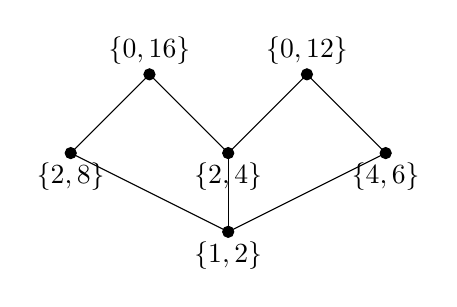
\begin{tikzpicture}
			\filldraw[black] (0,0) circle(2pt) node[anchor=north]{$\{1,2\}$};
			\filldraw[black] (-2,1) circle(2pt) node[anchor=north]{$\{2,8\}$};
			\filldraw[black] (0,1) circle(2pt) node[anchor=north]{$\{2,4\}$};
			\filldraw[black] (2,1) circle(2pt) node[anchor=north]{$\{4,6\}$};
			\filldraw[black] (-1,2) circle(2pt) node[anchor=south]{$\{0,16\}$};
			\filldraw[black] (1,2) circle(2pt) node[anchor=south]{$\{0,12\}$};
			\draw[black] (0,0)--(0,1);
			\draw[black] (0,0)--(-2,1);
			\draw[black] (0,0)--(2,1);
			\draw[black] (-2,1)--(-1,2);
			\draw[black] (2,1)--(1,2);
			\draw[black] (0,1)--(-1,2);
			\draw[black] (0,1)--(1,2);
		\end{tikzpicture}
	\end{center}
	$(S,\sigma)$ non è quindi un reticolo in quanto possiamo vedere che esistono in $(B,\sigma)$ due elementi massimali.
	\item Preso $C=\{\{1,2\},\{2,8\},\{2,4\},\{0,16\}\}$ di cardinalità 4 abbiamo che $0 = min(C,\sigma) = \{1,2\}$ e $1 = max(C,\sigma) = \{0,16\}$ e per ogni $x \in C \bigl(\exists y \in C (x \vee y = 1 \land x \wedge y = 0)\bigr)$, ovvero $(C,\sigma)$ è complementato.
	\item Abbiamo $\{\{1,4\}\}^{\downarrow} = \{\{1,-1\},\{1,4\}\}$. Inoltre: $\{1,4\} \wedge \{1,6\}=\{1,-1\}$ mentre $\{1,4\} \vee \{1,6\} = \{0,12\}$.
	\item Il minimo di $(A,\sigma)$ è rappresentato dalla parte $\{1,-1\}$. Esistono poi infiniti elementi massimali che sono le parti del tipo $\{0,a\}$, con $a \in \mathbb{Z}\setminus\{0\}$. Una parte $\{0,a\}$, infatti, non può essere seguita da alcun elemento di $A$ in quanto 0 non divide nessun elemento di $\mathbb{Z}$.
	\item Dato che una parte del tipo $a=\{0,x\}$ è massimale in $(A,\sigma)$ non è possibile inserire un elemento $a$ tale che $(B \cup \{a\},\sigma)$ possa diventare un reticolo.
\end{enumerate}
\subsection*{Esercizio 2}
Controlliamo per quali valori di $c \in \{1,3,20,24,55,60\}$ l'equazione $470x \equiv_{350} 3c$ ammette soluzioni. Chiaramente deve essere $d = MCD(470,350) \divides 3c$. Ovvero $d=10 \divides 3c$. Vera solo per $c=20$ e $c=60$. Abbiamo allora:
\begin{itemize}
	\item Sia $c=20$, allora l'equazione diventa: $470x \equiv_{350} 60$. Dividendo tutto per 10 si ottiene l'equazione equivalente $47x \equiv{35} 6$. È possibile scrivere $1=MCD(47,35)$ come combinazione lineare $1=47\cdot(3)+35\cdot(-4)$. Moltiplicando tutto per 6 abbiamo: $6=47 \cdot (18)+35 \cdot(-24)$. Quindi $x=[18]_{35}$ è una soluzione dell'equazione. Ovvero, l'insieme dei numeri interi $\{n \in \mathbb{Z} \; | \; n = 35k+18 \}$.
	\item Sia $c=60$. L'equazione diventa: $470x \equiv_{350} 180$. Dividendo per 10 otteniamo: $47x \equiv_{35} 18$. Moltiplicando nuovamente $1=47\cdot(3)+35\cdot(-4)$ per 18 si ha che $x=[54]_{35}=[19]_{35}=\{n \in \mathbb{Z} \; | \; n=35k+19 \}$.
\end{itemize}
\subsection*{Esercizio 3}
\begin{enumerate}[label=(\textit{\roman*})]
	\item Il numero di $8$-parti di $S$ è dato dal calcolo del coefficiente binomiale di 13 su 8:
	\begin{align*}
		\binom{13}{8} &= \frac{13!}{8!(13-8)!}\\
		&=\frac{13!}{8! \cdot 5!} \\
		&= \frac{13 \cdot 12 \cdot 11 \cdot 10 \cdot 9 \cdot 8 \cdot 7 \cdot 6 \cdot 5 \cdot 4 \cdot 3 \cdot 2 \cdot 1}{(8 \cdot 7 \cdot 6 \cdot 5 \cdot 4 \cdot 3 \cdot 2 \cdot 1)(5 \cdot4 \cdot 3 \cdot 2 \cdot 1)} \\
		&= \frac{13 \cdot 12 \cdot 11 \cdot 10 \cdot 9 \cdot \cancel{8 \cdot 7 \cdot 6 \cdot 5 \cdot 4 \cdot 3 \cdot 2 \cdot 1}}{(\cancel{8 \cdot 7 \cdot 6 \cdot 5 \cdot 4 \cdot 3 \cdot 2 \cdot 1})(5 \cdot4 \cdot 3 \cdot 2 \cdot 1)} = \\
		&=\frac{13 \cdot 12 \cdot 11 \cdot 10 \cdot 9}{5 \cdot4 \cdot 3 \cdot 2 \cdot 1}\\
		&=1287
	\end{align*}
	\item Non esistono parti di $S$ di cardinalità 18.
	\item Fissato $h$ in $T$ restano da essere selezionati altri 6 elementi dall'insieme $S$ che contiene ora $13-1$ elementi disponibili. Il numero di parti di $S\setminus\{h\}$ di sei elementi è dato da:
	\begin{align*}
		\binom{12}{6} = \frac{12!}{6!(6!)} = 924
	\end{align*}
	\item Una relazione binaria in $S$ è una delle qualsiasi parti di $S \times S$, che è noto avere $13^{2}$ elementi, ovvero 169 elementi.
\end{enumerate}
\subsection*{Esercizio 4}
Osserviamo che $\ast$ non è associativa in $\mathbb{Z}$. Infatti, presa la terna $(1,2,1)$ osserviamo che $(1 \ast 2) \ast 1 = 3+6+1=10$ mentre $1 \ast (2 \ast 1) = 9+6+1=16$. Possiamo quindi affermare che $(\mathbb{Z},\ast)$ è un gruppoide. Stesso discorso in $\mathbb{Z}_{6}$ in quanto:
\begin{align*}
	\forall a,b,c \in \mathbb{Z}_{6} \bigl( a \ast (b \ast c) = a \ast (3b +c) = 3a + 9b + 3c = 3a + 3b + 3c\bigr)
\end{align*}
mentre:
\begin{align*}
	\forall a,b,c \in \mathbb{Z}_{6} \bigl( (a \ast b) \ast c) = (3a+b) \ast c = 9a+3b+c = 3a+3b+c \bigr)
\end{align*}
Che in generale non coincidono. Al contrario, in $\mathbb{Z}_{3}$ abbiamo che:
\begin{align*}
	(a \ast b) \ast c = (3a+b) \ast c = b \ast c = 3b+c = c \\
	a \ast (b \ast c) = a \ast (3b+c) = a \ast c = 3a+c = c
\end{align*}
Quindi $(Z_{3},\ast)$ risulta essere un semigruppo. Verifichiamo quindi la commutatività in $\mathbb{Z}_{3}$:
\begin{align*}
	\forall a,b \in \mathbb{Z}_{3}(a \ast b \stackrel{?}{=} b \ast a)
\end{align*}
Abbiamo:
\begin{align*}
	a \ast b = 3a+b=b\\
	b \ast a = 3b+a=a
\end{align*}
Quindi $\ast$ non è commutativa. Studiamo l'eventuale esistenza di elementi neutri a sinistra o a destra. Un elemento $t$ è neutro a sinistra se:
\begin{align*}
	\forall x \in \mathbb{Z}_{3} \bigl(t \ast x \equiv_{3} x\bigr) &\iff 	\forall x \in \mathbb{Z}_{3} \bigl(3t+x \equiv_{3} x\bigr) \\
	\forall x \in \mathbb{Z}_{3} \bigl(3t \equiv_{3} 0 \bigr)
\end{align*}

Trovando quindi che tutti gli elementi di $\mathbb{Z}_{3}$ risultano essere elementi neutri a sinistra. Verifichiamo l'esistenza di elementi neutri a destra. Un elemento è neutro a destra se:
\begin{align*}
	\forall x \in \mathbb{Z}_{3} \bigl(x \ast t \equiv_{3} x\bigr) &\iff 	\forall x \in \mathbb{Z}_{3} \bigl(3x+t \equiv_{3} x\bigr) \\
	\forall x \in \mathbb{Z}_{3} \bigl(t \equiv_{3} x\bigr)
\end{align*}
Dato che $t$, per essere neutro a destra, deve coincidere con l'elemento $x$ col quale vogliamo comporlo per ottenere $x$ stesso, possiamo concludere dicendo che non esiste un elemento neutro a destra. Dato che un monoide è una struttura dotata di un elemento neutro a destra e a sinistra possiamo dire che $(\mathbb{Z}_{3},\ast)$ non è un monoide.
\subsection*{Esercizio 5}
\begin{enumerate}[label=(\textit{\roman*})]
	\item Abbiamo:
	\begin{align*}
		\overleftarrow{f}(\{10\})&=\{n \in S \; | \; f(n)=10\} \\
		&= \{n \in S \; | \; \sum_{n \geq p \in \mathbb{P}} p = 10 \} \\
		&= \{n \in S \; | \; 2+3+5=10=f(n) \} \\
		&= \{5,6\}
	\end{align*}
	Analogamente:
	\begin{align*}
		\overleftarrow{f}(\{11\})&=\{n \in S \; | \; f(n)=11\} \\
		&= \{n \in S \; | \; \sum_{n \geq p \in \mathbb{P}} p = 11 \} = \emptyset
	\end{align*}
	Infatti nella successione delle somme $f(n)$ abbiamo:
	\begin{equation}
		\Sigma_{n} = (f(n))_{n \in S} =  \{2,5,10,17,28,\ldots\} 
	\end{equation}
	Ogni termine della successione può essere ottenuto dalla formula ricorsiva $f(n) = f(n-1)+p_{n}$.
	\item Poiché $\overleftarrow{f}(\{10\})\geq 1$ possiamo dire che l'applicazione non è iniettiva. Analogamente, essendo $\overleftarrow{f}(\{11\})= \emptyset$, possiamo dire che $f$ non è suriettiva, e quindi biettiva.
	\item Si ha:
	\begin{align*}
		[8]_{\mathfrak{R}} &= \overleftarrow{f}(\{f(8)\}) = \overleftarrow{f} (\{17\}) = \{7,8,9,10\}
	\end{align*}
	\item Osserviamo che $S/{\mathfrak{R}}$ è l'insieme delle classi di equivalenza $[n]_{\mathfrak{R}}$, ovvero partizione composta dalle parti:
	\begin{align*}
		\bigl\{\overleftarrow{f}(\{f(n)\}) \; | \; n \in S \bigr\} = \bigl\{\overleftarrow{f}(\{\Sigma_{n}\}) \; | \; n \in S \bigr\}
	\end{align*}
	Dato che la successione $(\Sigma_{n})_{n \in S}$ risulta essere infinita abbiamo che $S/{\mathfrak{R}}$ è infinito.
	\item Abbiamo che $T/{\mathfrak{R}_{T}}$ è composto dalle classi:
	\begin{itemize}
		\item $[10]_{\mathfrak{R}_{T}}=\overleftarrow{f}(\{f(10)\}) = \overleftarrow{f}(\{17\}) = \{10\}$
		\item $[11]_{\mathfrak{R}_{T}}=\overleftarrow{f}(\{f(11)\}) = \overleftarrow{f}(\{28\}) = \{11,12\}$
		\item $[13]_{\mathfrak{R}_{T}}=\overleftarrow{f}(\{f(13)\}) = \overleftarrow{f}(\{41\}) = \{13,14,15,16\}$
		\item $[17]_{\mathfrak{R}_{T}}=\overleftarrow{f}(\{f(17)\}) = \overleftarrow{f}(\{58\}) = \{17,18\}$
		\item $[19]_{\mathfrak{R}_{T}}=\overleftarrow{f}(\{f(19)\}) = \overleftarrow{f}(\{77\}) = \{19,20\}$
	\end{itemize}
	E vale $|T/{\mathfrak{R}_{T}}|=5$.
\end{enumerate}
\subsection*{Esercizio 6}
\begin{enumerate}[label=(\textit{\roman*})]
	\item Si ha:
	\begin{enumerate}[label=(\arabic*)]
		\item Vero.
		\item Falso.
		\item Vero.
	\end{enumerate}
	\item Consideriamo l'anello booleano $(\mathbb{Z}_{2},+,\cdot)$. Chiaramente, essendo ogni suo elemento idempotente, il polinomio $x^{2}+x=0$ ammette infinite radici date dalla classe di equivalenza $\overline{0}_{2}$.
	\item Abbiamo:
	\begin{enumerate}
		\item $f$ non ha divisori monici di grado 3;
		\item $f$ ha un solo divisore monico di grado 2 che è il polinomio $upq$ associato al polinomio $pq$.
		\item Un divisore di grado $5$ può essere ottenuto eseguendo il prodotto tra $pr$ o $qr$. Tali polinomi avranno un polinomio monico associato. Moltiplicando un divisore monico per un elemento non nullo di $\mathbb{Z}_{13}$​ otteniamo un divisore non monico, e ci sono 12 possibili moltiplicatori (elementi di $\mathbb{Z}_{13})$. Si ottengono quindi 24 polinomi di grado 5, monici e non monici, che dividono $f$.
	\end{enumerate}
\end{enumerate}
\vfill
\section{Esame del 10 settembre 2024}
\begin{center}
	\includegraphics[scale=.85]{pdf/24-09-10.pdf}
\end{center}
\subsection*{Esercizio 1}
Costruiamo la tavola di verità:
\begin{center}
	\begin{tblr}
		{
			hlines,
			vlines,
			row{1}={primary!40!white},
			colspec={cccccX[c]X[c]},
			cells={mode=math}
		}
	p & q & r & p \implies q & q \implies r & p \implies (q \implies r) & (p \implies q) \implies r \\
	V & V & V & V & V & V & V \\
	V & V & F & V & F & F & F \\
	V & F & V & F & V & V & V \\
	V & F & F & F & V & V & V\\
	F & V & V & V & V & V & V\\
	F & V & F & V & F & V & F\\
	F & F & V & V & V & V & V\\
	F & F & F & V & V & V & F\\
	\end{tblr}
\end{center}
Le ultime due colonne non sono equivalenti e quindi possiamo affermare che non vale la proprietà associativa per l'implicazione.
\subsection*{Esercizio 2}
\begin{enumerate}[label=(\textit{\roman*})]
	\item L'operazione $\ast$ è associativa. Presi infatti tre elementi $a,b,c \in \mathbb{Z}_{12}$ abbiamo:
	\begin{align*}
		a \ast (b \ast c) &= a \ast (b+9c) \\
		&= a+ 9(b+9c) \\
		&= a+9b +81c \\
		&= a+9b+9c & \text{\textcolor{gray}{(In quanto $\overline{81}\equiv_{12} \overline{9}$)}}\\
\end{align*}
		\begin{align*}
		(a \ast b) \ast c = (a+9b) \ast c = a +9b+9c
	\end{align*}
	L'operazione $\ast$ non è commutativa, infatti presi $a=\overline{0}$ e $b=\overline{1}$ abbiamo $\overline{0} \ast \overline{1} = \overline{9}$ e $\overline{1} \ast \overline{0} = \overline{1}$. Un eventuale elemento neutro a sinistra $t$ deve rendere vera l'uguaglianza $t \ast a =  a$ per ogni $a \in \mathbb{Z}_{12}$, ossia:
	\begin{align*}
		t \ast a = a &\iff t +9a = a \\
		&\iff t =-8a
	\end{align*}
Quindi, dovendo $t$ dipendere da $a$, possiamo concludere che non esiste un siffatto elemento neutro a sinistra. Cerchiamo ora un elemento neutro a destra. Sempre per definizione di elemento neutro a destra, per ogni $a \in \mathbb{Z}_{12}(a \ast t = a)$:
\begin{align*}
	a \ast t = a &\iff a +9t = a \\
	&\iff 9t = 0 \\
	&\iff t=\overline{0} \lor t = \overline{4} \lor t = \overline{8}
\end{align*}
Non esistendo un $t$ che sia neutro sia a sinistra che a destra possiamo affermare che $(\mathbb{Z}_{12},\ast)$ è un semigruppo.
\item Abbiamo $D=\{\overline{0},\overline{4},\overline{8}\}$, $S=\emptyset$. Quindi $D \cup S = D$. Verifichiamo se $D=\{\overline{4n}\;|\; n \in \mathbb{Z}\}$ è stabile. Siano $x=4n, \ y=4m  \in D$, vale allora:
\begin{align*}
	4n \ast 4m &= 4n + 9 \cdot 4m \\
	&= 4n + 36m \\
	&= 4n 
\end{align*}
Quindi $D$ è stabile.
\item Abbiamo $T=\{\overline{0},\overline{3},\overline{6},\overline{9}\}$. Ogni $x \in T$ è esprimibile come $3n$ per un opportuno intero $n$. Siano $x =3n,\ y=3m \in T$, vale allora:
\begin{align*}
	3n \ast 3m &= 3n + 9 \cdot 3m \\
	&= 3n + 27m \\
	&= 3n + 3m \\
	&= 3(n+m)
\end{align*}
Quindi $T$ è stabile. L'operazione $\ast$ in $T$ è commutativa e $\overline{0}$ risulta elemento neutro. Inoltre, per ogni $x \in T$ esiste un simmetrico $x'$ tale che $x \ast x' = 0$. Infatti, posto $x =3n$ e $x'=3m$:
\begin{align*}
	x \ast x' = 0 &\iff 3n \ast 3m = 0 \\
	&\iff 3n + 3m = 0 \\
	&\iff 3m = -3n \\
	&\iff 3m = -3n+12 \\
	&\iff 3m = -3(n-12) \\
	&\iff 3m = 3(4-n)
\end{align*}
Quindi $x'\in T$ e $(T,\ast)$ è un gruppo abeliano.
\item Risolviamo:
\begin{align*}
	\overline{7} \ast x \equiv_{12} 1 &\iff 7 + 9x \equiv_{12} 1 \\
	&\iff 9x \equiv_{12} -6 \\
	&\iff 9x \equiv_{12} 6
\end{align*}
Calcoliamo $(9,12)=3$, poiché $3 \divides 6$ abbiamo tre soluzioni non congruenti. Riduciamo l'equazione congruenziale:
\begin{align*}
	3x \equiv_{4} 2 
\end{align*}
Dove $(3,4)=1$ e ovviamente $1=4 + 3(-1)$. Moltiplicando tale combinazione lineare otteniamo $2 = 4(2) + 3(-2)$. Quindi $x=-2 = 2$ è soluzione di tale equazione. Ritornando al modulo 12, abbiamo le tre soluzioni:
\begin{align*}
	x = 2 + k\frac{12}{3} = 2 + 4k
\end{align*}
con $0 \leq k < 3$. Sia ora:
\begin{align*}
	5 \ast x \equiv_{12} 1 &\iff 5+9x \equiv_{12} 1 \\
	&\iff 9x \equiv_{12} -4 \\
	&\iff 9x \equiv_{12} 8
\end{align*}
Calcoliamo $(9,12)=3$, e 3 non divide 8, quindi non esistono soluzioni.
\end{enumerate}
\subsection*{Esercizio 3}
\begin{enumerate}[label=(\textit{\roman*})]
	\item La funzione $\varphi$ è suriettiva. Infatti, ogni intero $n \in \mathbb{Z}$ è immagine di almeno un polinomio. Preso lo $0$ ad esempio sappiamo che qualunque polinomio non completo $f$ ha come immagine $\varphi(f) = 0$. Inoltre, preso un qualsiasi $n \in \mathbb{Z}$, questo ammette una fattorizzazione in primi $n = p_{0}^{\alpha_{0}} \cdot \ldots p_{n}^{\alpha_{n}}$ dal quale possiamo ottenere il polinomio:
	\begin{align*}
		f =p_{0}^{\alpha_{0}} + p_{1}^{\alpha_{1}}x + \ldots + p_{n}^{\alpha_{n}}x^{n}
	\end{align*}
	Ed ovviamente  $\varphi(f)=n$. Ovviamente stando in $\mathbb{Z}$, la fattorizzazione di un intero non è unica. Ad esempio $24 = (3)(2^{3}) = (-3)(-2)^{3}$ ottenendo così i due polinomi distinti, ma associati:
	\begin{align*}
		f_{1}=3x^{3}+2x^{2}+2x+2\\
		f_{2}=-3x^{3}-2x^{2}-2x-2
	\end{align*}
e vale $\varphi(f_{1})=\varphi(f_{2})=24$.
	\item Abbiamo:
	\begin{itemize}
		\item $\overrightarrow{\varphi}(\{1,x^{5}+1\})=\{\varphi(1),\varphi(x^{5}+0x^{4}+0x^{3}+0x^{2}+0x+0)\}=\{1,0\}$.
		\item $\overleftarrow{\varphi}(\{3\})$ è l'insieme $\{3x+1,-3x-1,3,f_{n,3}\}$ dove $f_{n,3}$ è un polinomio di grado $n$ tale che $\Pi_{i=0}^{n-1} a_{i}= 1$ e $a_{n}=3$, al variare di $n \in \mathbb{Z}$;
		\item $\overleftarrow{\varphi}(\{2,4\})$ è l'insieme $\{2x+1,-2x-1,2,f_{n,2}\}$ dove $f_{n,2}$ è un polinomio $\{a_{n}\}_{n \in \mathbb{N}}$ tale che $\Pi_{i=0}^{n-1} a_{i} = 1$ e $a_{n}=2$, unito all'insieme dei polinomi $\{4,4x+1,2x+2,-2x-2,f_{n,4}\}$ dove $f_{n,4}$ è un polinomio $\{a_{n}\}_{n \in \mathbb{N}}$ e $\Pi_{i=0}^{n-1} a_{i} = 1$ e $a_{n}=4$.
	\end{itemize}
	 In $\mathbb{Q}[x]$ il polinomio $x+3$ ed il suo associato $(-x-3)$ risultano essere polinomi irriducibili di primo grado appartenenti a $\overleftarrow{\varphi}(\{3\})$, così come il polinomio $(-3x-1)$ e $(3x+1)$.
	\item Per quanto osservato nei punti precedenti è ovvio che ogni classe di equivalenza $[f]_{\mathfrak{R}_{\varphi}}$ risulta essere infinita in quanto è sempre possibile costruire un polinomio $g$ tale che $\varphi(g)=\varphi(f)$ sommando un termine con coefficiente 1.
	\item Due polinomi $f$ e $g$ di $A[x]$ si dicono associati se e solo se $f \divides g \land g \divides f$. Sempre per i punti precedenti abbiamo visto che, poiché in $\mathbb{Z}$ non è unica la fattorizzazione, è sempre possibile costruire due polinomi associati appartenenti alla stessa classe di equivalenza.
\end{enumerate}
\subsection*{Esercizio 4}
\begin{enumerate}[label=(\textit{\roman*})]
	\item La relazione $\rho_{A}$ non è una relazione d'ordine in quanto $2 \ \rho_{A} \ 14 \land 14 \ \rho_{A} \ 2$ ma $2 \neq 14$.
	\item Posto $\rho = \rho_{B}$ abbiamo:
	\begin{itemize}
		\item Ogni elemento è in relazione con 0
		\item L'elemento 2 è in relazione con 132, 330,0
		\item L'elemento -3 è in relazione con 132, 330, 0 
		\item L'elemento 11 è in relazione con 132, 330, 0
		\item L'elemento 49 è in relazione 0
		\item L'elemento 132 è in relazione con 0
		\item L'elemento 330 è in relazione 0
	\end{itemize}
Quindi:
\begin{center}
	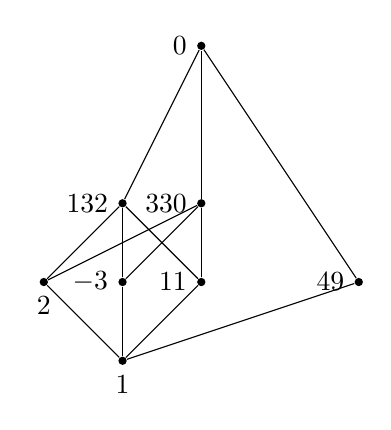
\begin{tikzpicture}
			\node[circle,fill=black,inner sep=0pt,minimum size=3pt,label=below:{$1$}](a) at (1,0){};
		\node[circle,fill=black,inner sep=0pt,minimum size=3pt,label=below:{$2$}](b) at (0,1){};
		\node[circle,fill=black,inner sep=0pt,minimum size=3pt,label=left:{$-3$}](c) at (1,1){};
		\node[circle,fill=black,inner sep=0pt,minimum size=3pt,label=left:{$11$}](d) at (2,1){};
		\node[circle,fill=black,inner sep=0pt,minimum size=3pt,label=left:{$49$}](e) at (4,1){};
		\node[circle,fill=black,inner sep=0pt,minimum size=3pt,label=left:{$132$}](f) at (1,2){};
		\node[circle,fill=black,inner sep=0pt,minimum size=3pt,label=left:{$330$}](g) at (2,2){};
		\node[circle,fill=black,inner sep=0pt,minimum size=3pt,label=left:{$0$}](h) at (2,4){};
		\draw[thin,black](a)--(b);
		\draw[thin,black](a)--(c);
		\draw[thin,black](a)--(d);
		\draw[thin,black](a)--(e);
		\draw[thin,black](b)--(f);
		\draw[thin,black](c)--(f);
		\draw[thin,black](d)--(f);
		\draw[thin,black](b)--(g);
		\draw[thin,black](c)--(g);
		\draw[thin,black](d)--(g);
		\draw[thin,black](g)--(h);
		\draw[thin,black](f)--(h);
		\draw[thin,black](e)--(h);
	\end{tikzpicture}
\end{center}
	\item Abbiamo che $2 \wedge 49 = 1$ mentre $2 \vee 49 = 0$.
	\item $(B,\rho)$ è un reticolo complementato non distributivo in quanto possiamo osservare l'esistenza di un sottoreticolo isomorfo al reticolo pentagonale.
\end{enumerate}
\subsection*{Esercizio 5}
Un grafo semplice è un grafo non orientato. Una coppia $G=(V,R)$ è un grafo se e solo se $V$ è un insieme non vuoto ed $R$ risulta essere una relazione binaria in $V$ tale che $R$ sia antiriflessiva e simmetrica. Nel caso in esame la relazione in $V \subseteq \mathbb{N}^{*} \setminus \{1\}$ risulta essere antiriflessiva in quanto $\forall a \in V \bigl((a,a)=a\bigr)$ e inoltre se $(a,b)=1$ allora anche $(b,a)=1$.
\begin{enumerate}[label=(\textit{\roman*})]
	\item Se $V=\mathbb{N}^{*}$ la relazione $R$ non risulta essere antiriflessiva in quanto 1 è coprimo con se stesso.
	\item Ogni numero non è adiacente con i suoi multipli. Preso un multiplo $m$ di elemento $a \in \mathbb{N}^{*} \setminus \{1\}$ tale multiplo risulterà essere coprimo con un elemento $b$, coprimo con $a$, a meno che $m$ non sia multiplo del minimo comune multiplo tra $a$ e $b$, quindi possiamo essere. In generale, presa una fattorizzazione di $m$, tale numero sarà coprimo con ogni primo non appartenente alla sua fattorizzazione e tale primo sarà coprimo con ogni primo della fattorizzazione di $m$, quindi è sempre possibile trovare un percorso tra un numero e l'altro. Quindi $G_{V}$ è connesso.
	\item Sia $V=\{2,3,4,12\}$, chiaramente 12 è un vertice isolato e quindi $V$ non risulta essere connesso.
	\item $V$ non ha circuiti euleriani in quanto $deg(5)$ non è pari.
\end{enumerate}


\section{Esame del 19 giugno 2025}
\begin{center}
    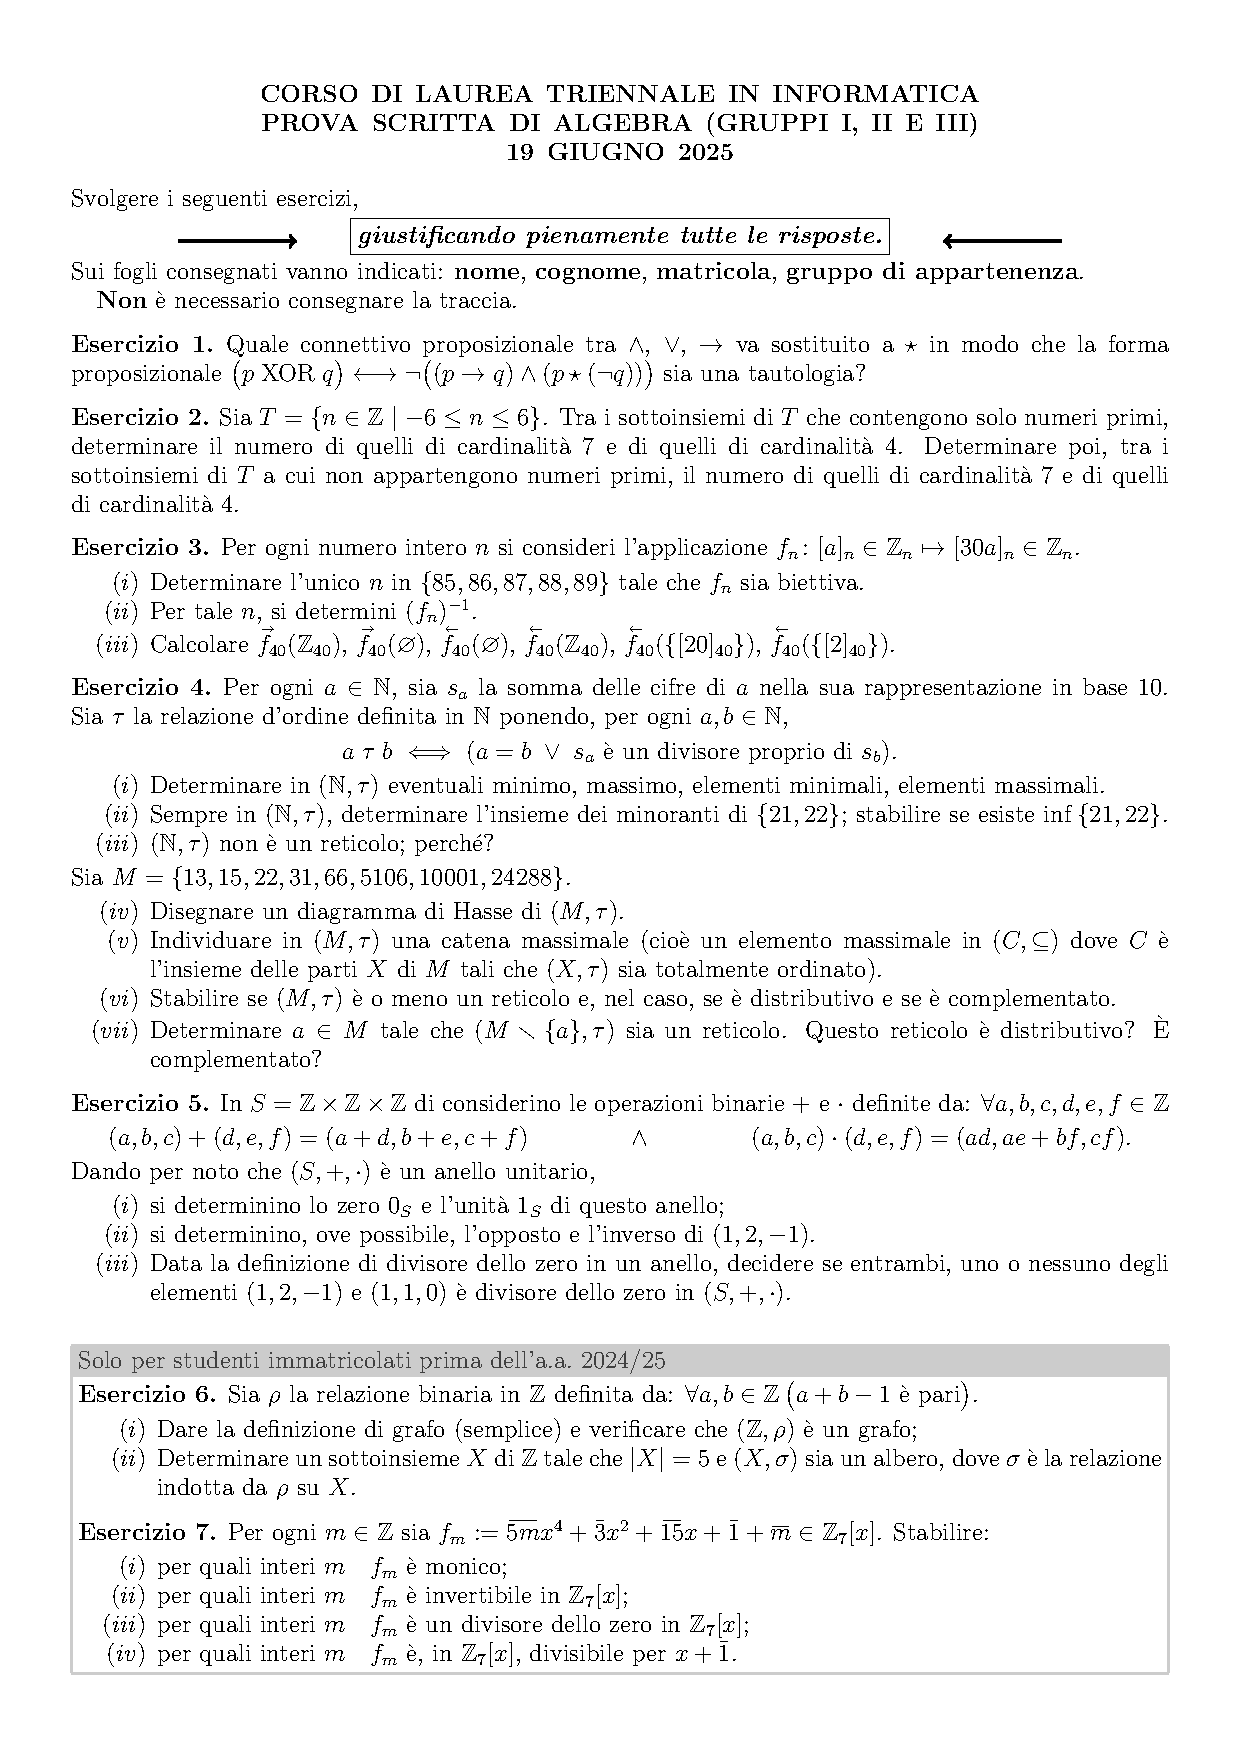
\includegraphics[scale=.85]{pdf/25-06-19.pdf}
\end{center}

\subsection*{Esercizio 1}
Ok dobbiamo capire per quale $\star$ sia una tautologia, cerchiamo di avere già tutti i valori pronti e poi proviamo AND, OR e $\implies$ per capire chi potrebbe dare una tautologia.
\begin{center}
    \begin{tblr}
        {
            hlines,
            vlines,
            row{1}={primary!40!white},
            colspec={cccccX[c]X[c]},
            cells={mode=math}
        }
    p & q & p \oplus q & ( p \implies q ) & ( p \land \neg(q) ) & \neg ( ( p \implies q ) \land ( p \land \neg(q) ) ) \\
    V & V & F & V & V & V \\
    V & V & V & F & V & F \\
    F & V & V & V & F & F \\
    F & F & F & V & V & V\\
    \end{tblr}

Se compariamo l'ultima colonna (a cui già abbiamo applicato il NOT) con quella dello XOR ci accorgiamo che hanno gli stessi valori, abbiamo una tautologia!
\end{center}

\subsection*{Esercizio 2}
Esplicitiamo i numeri primi in T: $S = \{-5, -3, -2, 2, 3, 5\}$ \\
Cardinalità 7: $\emptyset$. Ovvio perché l'insieme ha 6 elementi come possiamo raggrupparlo per 7? \\
Cardinalità 4: $\binom{6}{4} = \frac{6!}{4!(2!)} = \frac{6 \cdot 5}{2} = 15$. \\
Creiamo un nuovo insieme per "Determinare poi, tra i sottoinsiemi di T a cui non appartengono numeri primi" \\
$H: T \setminus S = \{-6, -4, -1, 0, 1, 4, 6\}$ \\
Cardinalità 7: $\binom{7}{7} = 1$ \\
Cardinalità 4: $\binom{7}{4} = \frac{7!}{4!(3!)} = \frac{7 \cdot 6 \cdot 5}{3 \cdot 2 \cdot 1} = 35$ \\

\subsection*{Esercizio 3}
Utilizzando il lemma che ci dice che quando 30 ed n sono coprimi allora sono invertibili sappiamo già che n = 89 ci renderà fn biettiva.

\vspace{1em}

$MCD(30,89) = 1$

\vspace{1em}

$89 = 30 \cdot 2 + 29 \implies 29 = 89 - 30 \cdot 2$

$30 = 29 \cdot 1 + 1 \implies 1 = 30 - 29$

$1 = 30 - (89 - 30 \cdot 2) \implies 30(1+2) - 89 \implies 30 \cdot 3 - 89$

$30 \cdot 3 \equiv 90 \pmod{89} \rightarrow [30 \cdot 3]_{89} = [1]_{89} \rightarrow [a]_{89} = [3]_{89}$

\begin{itemize}
    \item $\vec{f}_{40}(\mathbb{Z}_{40}) = \{[0]_{40}, [10]_{40}, [20]_{40}, [30]_{40}\}$.
    \item $\vec{f}_{40}(\emptyset) = \emptyset$.
    \item $\overleftarrow{f}_{40}(\emptyset) = \emptyset$.
    \item $\overleftarrow{f}_{40}(\mathbb{Z}_{40}) = \mathbb{Z}_{40}$.
    \item $\overleftarrow{f}_{40}(\{[20]_{40}\}) = \{[2]_{40}, [6]_{40}, [10]_{40}, [14]_{40}, [18]_{40}, [22]_{40}, [26]_{40}, [30]_{40}, [34]_{40}, [38]_{40}\}$.
    \item $\overleftarrow{f}_{40}(\{[2]_{40}\}) = \emptyset$.
\end{itemize}

\subsection*{Esercizio 4}

\subsubsection*{Primo punto}

Ok ragioniamoci un pò. Dice che dovremmo mettere in relazione la somma dell cifre dei numeri che si dividono tra loro. E
la somma di a è indicato come sA mentre la somma delle cifre di b come sB. Quindi avremo una relazione quando il numero
13 la cui somma fa 4 divider un altro numero ad esempio 17 perché 1 + 7 = 8. \\ \\ 

In un contesto "normale" senza giri strane con le somme quando un numero divide sempre TUTTI gli altri? Quando è 1, in questo
caso tutti i numeri che sono potenze di 10. $10^0 = 1, 10^1 = 10$ la cui somma fa 1, $10^2 = 100$ la cui somma fa 1 ecc\dots Quindi come
minimali abbiamo tutte le potenze di 10 e di conseguenza non esiste minimo. \\ \\

Quale numero invece viene diviso da tutti? 0 E in questo caso il massimo è anche massimale

\subsubsection*{Secondo punto}

$MINOR_{(\mathbb{N}, \tau)}(\{21, 22\}) = \{ m \in \mathbb{N} \mid \forall x \in \{21, 22\}, m \tau x \} = \{ m \in \mathbb{N} \mid Sm < 3 \}$
% Testo blu
INF $\{21, 22\}$ non può esistere perché è il MAX dei minoranti ma essendo che ce ne sono infiniti, non esisterà alcun INF

\subsubsection*{Terzo punto}

Non è un reticolo perché non può avere INF (visto che ci sono diversi minimali).

\subsubsection*{Quarto punto}

\begin{center}
    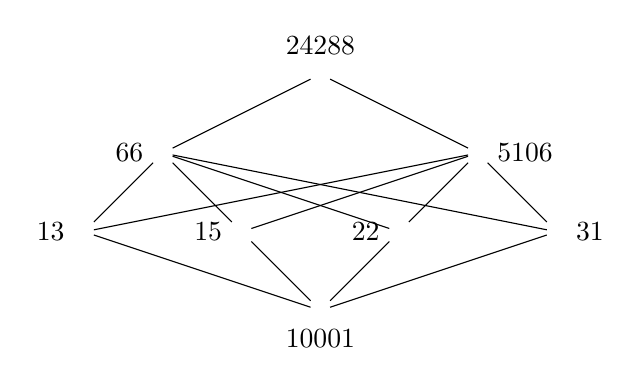
\begin{tikzpicture}
        % Nodi del livello più basso (10001)
        \node[label=below:{$10001$}](n10001) at (3,0) {}; % Posizionato al centro in basso

        % Nodi del livello intermedio (13, 15, 22, 31)
        \node[label=left:{$13$}](n13) at (0,1) {};
        \node[label=left:{$15$}](n15) at (2,1) {};
        \node[label=left:{$22$}](n22) at (4,1) {};
        \node[label=right:{$31$}](n31) at (6,1) {};

        % Nodi del livello superiore (66, 5106)
        \node[label=left:{$66$}](n66) at (1,2) {};
        \node[label=right:{$5106$}](n5106) at (5,2) {};

        % Nodi del livello più alto (24288)
        \node[label=above:{$24288$}](n24288) at (3,3) {};

        % Collegamenti da 10001 ai nodi del livello intermedio
        \draw (n10001)--(n13);
        \draw (n10001)--(n15);
        \draw (n10001)--(n22);
        \draw (n10001)--(n31);

        % Collegamenti da 13, 15, 22, 31 a 66
        \draw (n13)--(n66);
        \draw (n15)--(n66);
        \draw (n22)--(n66);
        \draw (n31)--(n66);

        % Collegamenti da 13, 15, 22, 31 a 5106
        \draw (n13)--(n5106);
        \draw (n15)--(n5106);
        \draw (n22)--(n5106);
        \draw (n31)--(n5106);

        % Collegamenti da 66 e 5106 a 24288
        \draw (n66)--(n24288);
        \draw (n5106)--(n24288);
    \end{tikzpicture}
\end{center}

Sì è un reticolo ed è complementato ma non distributivo.

\subsubsection*{Quinto punto}

\begin{center}
    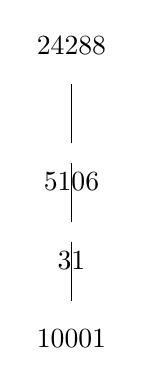
\begin{tikzpicture}
        % Nodi disposti verticalmente come nella figura
        \node[label=above:{$24288$}](n24288) at (0,3) {};
        \node[label=below:{$5106$}](n5106) at (0,2) {};
        \node[label=below:{$31$}](n31) at (0,1) {};
        \node[label=below:{$10001$}](n10001) at (0,0) {};

        % Collegamenti verticali
        \draw (n24288)--(n5106);
        \draw (n5106)--(n31);
        \draw (n31)--(n10001);
    \end{tikzpicture}
\end{center}

\subsubsection*{Sesto punto}

a = vuoto, vale tutto ciò che è stato detto al 4° punto.

\subsection*{Esercizio 5}

\subsubsection*{Punto 1}
L'elemento neutro rispetto alla somma è $\vec{0}_S = (0, 0, 0)$.
L'elemento neutro rispetto al prodotto è $\vec{1}_S = (0, 0, 1)$.

\subsubsection*{Punto 2}
Per l'elemento $(1, 2, -1)$, l'opposto è dato da $(a,b,c) + (a',b',c') = (0,0,0)$.
Per la prima componente: $1 + a' = 0 \implies a' = -1$.
Per la seconda componente: $2 + b' = 0 \implies b' = -2$.
Per la terza componente: $-1 + c' = 0 \implies c' = 1$.
Quindi, l'opposto di $(1, 2, -1)$ è $(-1, -2, 1)$.

L'inverso di $(1, 2, -1)$ deve soddisfare $(1, 2, -1) \cdot (a, b, c) = (0, 0, 1)$.
$(1 \cdot a, 1 \cdot b + 2 \cdot a, 1 \cdot c -1 \cdot a) = (a, b+2a, c-a) = (0, 0, 1)$.
$a=0$, $b+2a=0 \implies b=0$, $c-a=1 \implies c=1$.
L'inverso di $(1, 2, -1)$ è $(0, 0, 1)$.

\subsubsection*{Punto 3}
Per determinare se un elemento è un divisore dello zero, dobbiamo verificare se esiste un altro elemento non nullo che, moltiplicato per il primo, dà l'elemento neutro $(0,0,0)$.

Per $(1, 2, -1)$:
Supponiamo che esista un elemento $(a, b, c) \ne (0, 0, 0)$ tale che:
$(1, 2, -1) \cdot (a, b, c) = (a, b+2a, c-a) = (0, 0, 0)$.
Questo implica che:
$a = 0$
$b + 2a = 0 \implies b=0$
$c - a = 0 \implies c=0$
Quindi $(a, b, c) = (0, 0, 0)$. Non esiste un elemento non nullo che soddisfi la condizione, perciò $(1, 2, -1)$ **non** è un divisore dello zero.

Per $(1, 1, 0)$:
Supponiamo che esista un elemento $(a, b, c) \ne (0, 0, 0)$ tale che:
$(1, 1, 0) \cdot (a, b, c) = (a, b+a, c) = (0, 0, 0)$.
Questo implica che:
$a = 0$
$b + a = 0 \implies b=0$
$c = 0$
Quindi $(a, b, c) = (0, 0, 0)$. Anche in questo caso non esiste un elemento non nullo, quindi $(1, 1, 0)$ **non** è un divisore dello zero.

\section{Svolgimento Esame 16 Luglio}
\begin{center}
	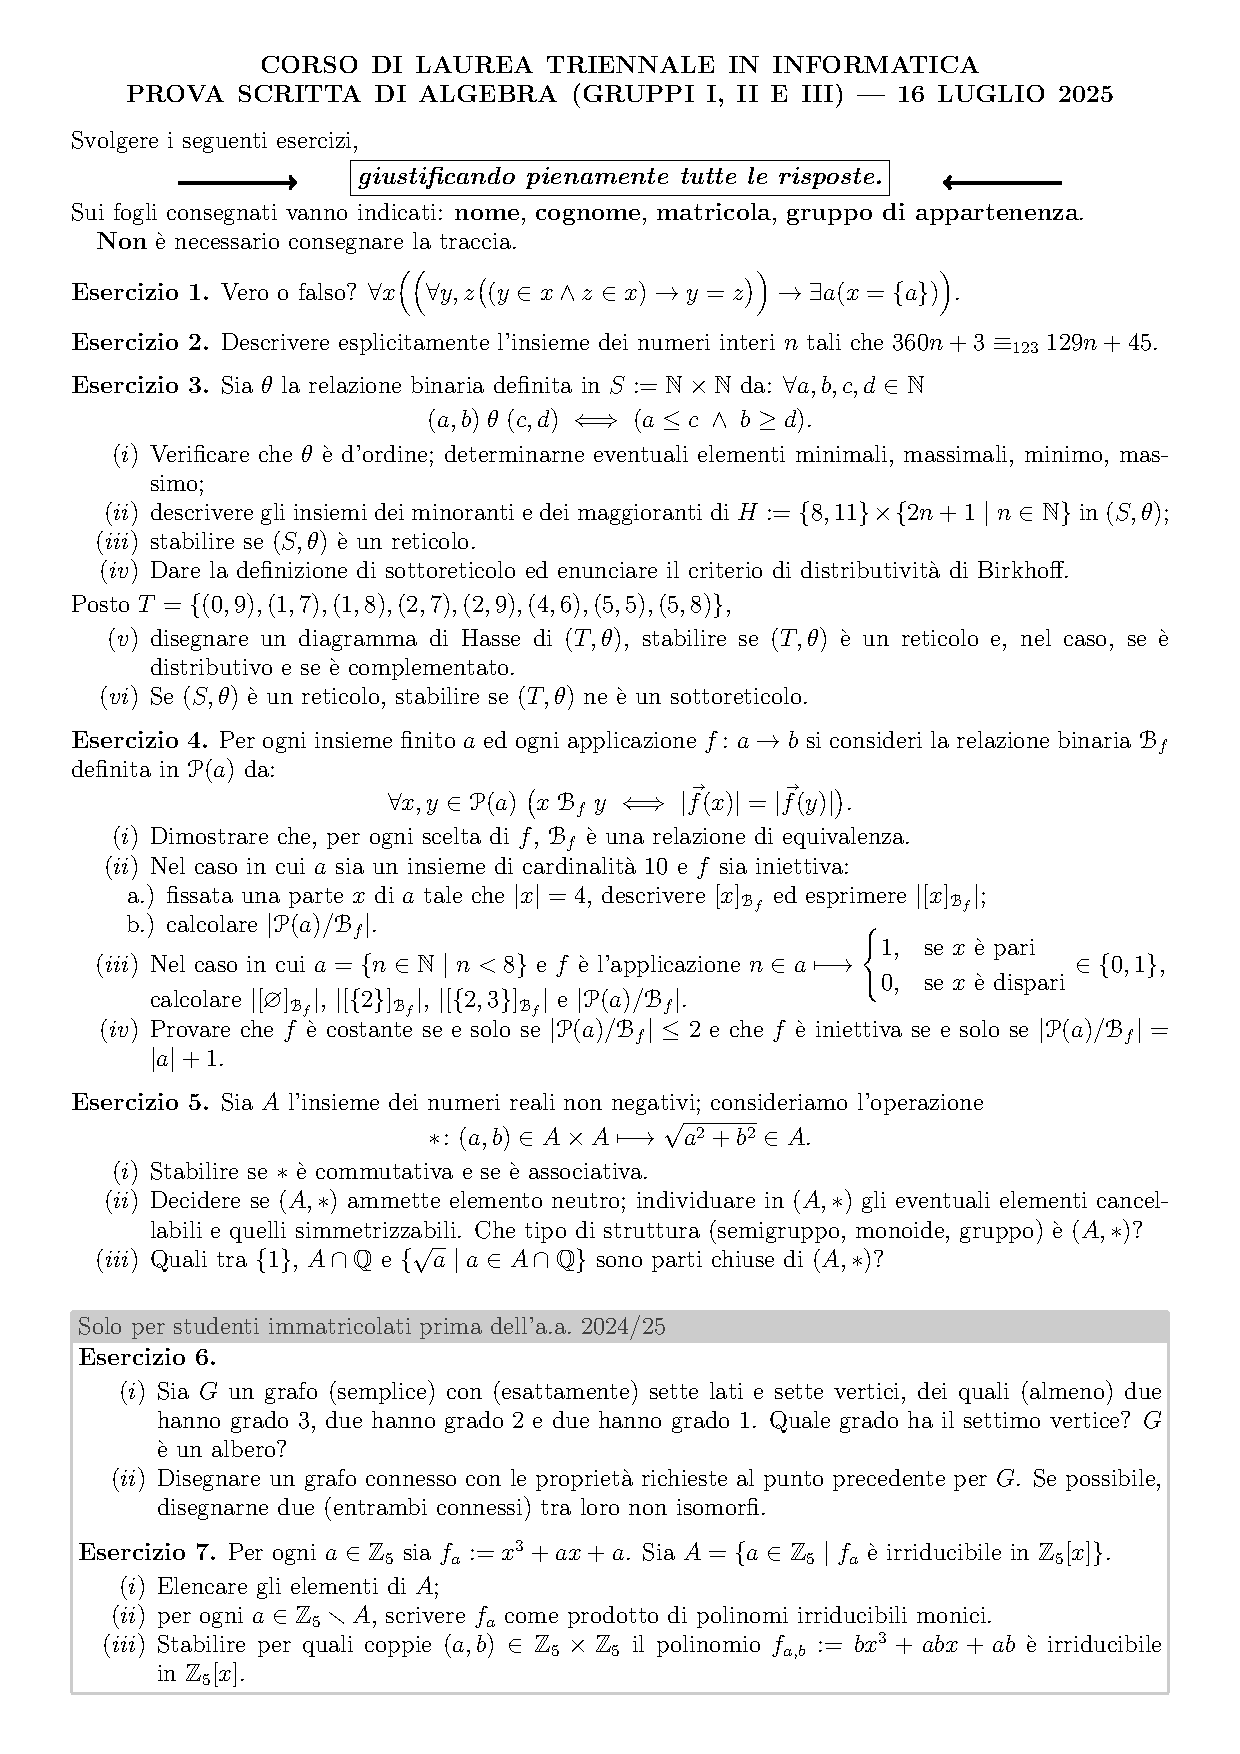
\includegraphics[scale=.85]{pdf/25-07-16.pdf}
\end{center}

\subsection*{Esercizio 1}
La proposizione $\forall x((\forall y,z((y\in x\wedge z\in x)\rightarrow y=z))\rightarrow\exists a(x=\{a\}))$ è falsa.
Per dimostrarlo, è sufficiente trovare un controesempio, cioè un insieme $x$ per cui la proposizione non è verificata.
Consideriamo l'insieme vuoto, $x = \emptyset$.
\begin{itemize}
    \item L'antecedente della prima implicazione, $(y\in x\wedge z\in x)$, è sempre falso perché non esistono elementi in $x$. Poiché l'antecedente è falso, l'implicazione $(y\in x\wedge z\in x)\rightarrow y=z$ è sempre vera.
    \item Di conseguenza, la proposizione quantificata $(\forall y,z((y\in x\wedge z\in x)\rightarrow y=z))$ è vera.
    \item Consideriamo ora il conseguente della seconda implicazione, $\exists a(x=\{a\})$. Se $x=\emptyset$, non esiste un elemento $a$ tale che $x=\{a\}$, quindi la proposizione è falsa.
\end{itemize}
La proposizione completa diventa quindi: $(\text{vero}) \rightarrow (\text{falso})$, che è falsa. Poiché non è vera per ogni $x$, la proposizione iniziale è falsa.

\subsection*{Esercizio 2}
Dobbiamo risolvere la congruenza $360n+3\equiv_{123}129n+45.$
\begin{itemize}
    \item Riscriviamo la congruenza: $360n - 129n \equiv 45 - 3 \pmod{123}$.
    \item Otteniamo: $231n \equiv 42 \pmod{123}$.
    \item Calcoliamo il Massimo Comun Divisore tra 231 e 123 utilizzando l'algoritmo di Euclide:
    \begin{itemize}
        \item $231 = 1 \cdot 123 + 108$
        \item $123 = 1 \cdot 108 + 15$
        \item $108 = 7 \cdot 15 + 3$
        \item $15 = 5 \cdot 3 + 0$
    \end{itemize}
    Il MCD è 3. Poiché $3$ divide 42, esistono soluzioni. Dividiamo per 3 tutti i termini della congruenza:
    \item $\frac{231}{3}n \equiv \frac{42}{3} \pmod{\frac{123}{3}}$
    \item $77n \equiv 14 \pmod{41}$.
    \item Per trovare $n$, dobbiamo calcolare l'inverso di $77 \pmod{41}$.
    $77 \equiv 36 \equiv -5 \pmod{41}$.
    Quindi, l'inverso di $-5 \pmod{41}$ è $8$, poiché $(-5) \cdot (-8) = 40 \equiv -1 \pmod{41}$. Oh, scusa, è $(-5) \cdot 8 = -40 \equiv 1 \pmod{41}$. Quindi l'inverso è $8$.
    \item Moltiplichiamo entrambi i membri della congruenza per 8:
    $8 \cdot 77n \equiv 8 \cdot 14 \pmod{41}$
    $1n \equiv 112 \pmod{41}$
    $112 = 2 \cdot 41 + 30$, quindi $112 \equiv 30 \pmod{41}$.
    \item Le soluzioni sono $n \equiv 30 \pmod{41}$.

\end{itemize}

\subsection*{Esercizio 3}
Sia la relazione binaria definita in $S:=\mathbb{N}\times\mathbb{N}$ da: $(a, b) \theta (c,d)\iff(a\le c\wedge b\ge d)$.
\begin{itemize}
    \item[(i)] \textbf{Verifica che è una relazione d'ordine:}
    \begin{itemize}
        \item \textbf{Riflessività:} $(a,b)\theta(a,b)$ è vero poiché $a\le a$ e $b\ge b$.
        \item \textbf{Antisimmetria:} Se $(a,b)\theta(c,d)$ e $(c,d)\theta(a,b)$, allora $a\le c$ e $b\ge d$, e $c\le a$ e $d\ge b$. Questo implica che $a=c$ e $b=d$, quindi $(a,b)=(c,d)$.
        \item \textbf{Transitività:} Se $(a,b)\theta(c,d)$ e $(c,d)\theta(e,f)$, allora $a\le c\le e$ e $b\ge d\ge f$. Questo implica che $a\le e$ e $b\ge f$, ovvero $(a,b)\theta(e,f)$.
    \end{itemize}
    La relazione è d'ordine. Non esistono elementi minimali, massimali, minimo o massimo, poiché per ogni $(a,b)$ esiste un elemento $(a-1, b+1)$ più piccolo e $(a+1, b-1)$ più grande, a meno che $a=0$.

    \item[(ii)] \textbf{Insiemi di minoranti e maggioranti di $H$:}
    Sia $H:=\{8,11\}\times\{2n+1|n\in\mathbb{N}\} = \{(8,1), (8,3), (8,5), \dots, (11,1), (11,3), (11,5), \dots\}$.
    \begin{itemize}
        \item \textbf{Minoranti:} L'insieme dei minoranti di $H$ è dato da $\{(a,b)\in S | (a,b)\theta(c,d) \forall (c,d)\in H\}$.
        Questo implica che $a\le c$ e $b\ge d$ per ogni $(c,d)\in H$. Per la prima componente, $a\le 8$ e $a\le 11$, quindi $a\le 8$. Per la seconda, $b\ge 2n+1$ per ogni $n\in\mathbb{N}$, il che è impossibile. L'insieme dei minoranti è l'insieme vuoto, $\emptyset$.
        \item \textbf{Maggioranti:} L'insieme dei maggioranti di $H$ è dato da $\{(a,b)\in S | (c,d)\theta(a,b) \forall (c,d)\in H\}$.
        Questo implica che $c\le a$ e $d\ge b$ per ogni $(c,d)\in H$. Questo è possibile per ogni coppie (a,b) t.c a >= 11 AND b <= 1
    \end{itemize}
    \item[(iii)] \textbf{È un reticolo?}
    No, $(S, \theta)$ non è un reticolo

	\item[(iv)] \textbf{Def sottoreticolo e Birkhoff} 
	La trovate nelle dispense

	\item[(v)] \textbf{Disegnare Hasse dell'insieme T:}
	
	\begin{center}
		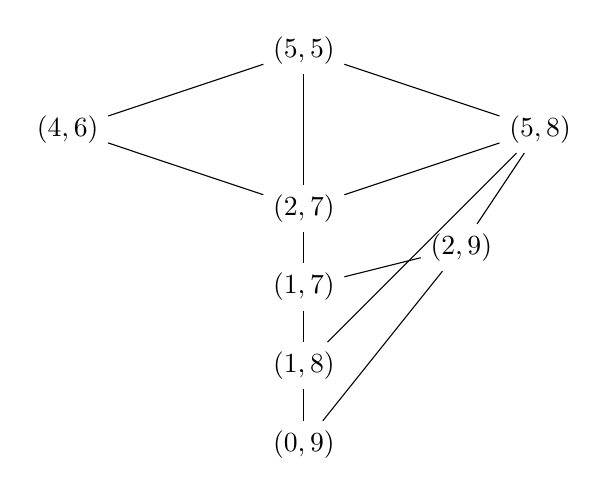
\begin{tikzpicture}
			% Nodi
			\node (n46) at (0,3) {$(4,6)$};
			\node (n55) at (3,4) {$(5,5)$};
			\node (n58) at (6,3) {$(5,8)$};
	
			\node (n27) at (3,2) {$(2,7)$};
			\node (n17) at (3,1) {$(1,7)$};
			\node (n18) at (3,0) {$(1,8)$};
			\node (n09) at (3,-1) {$(0,9)$};
			
			\node (n29) at (5,1.5) {$(2,9)$};
			
			% Collegamenti
			\draw (n46) -- (n27);
			\draw (n55) -- (n27);
			\draw (n58) -- (n27);
			
			\draw (n27) -- (n17);
			\draw (n17) -- (n18);
			\draw (n18) -- (n09);
			
			\draw (n58) -- (n29);
			\draw (n29) -- (n17);
			\draw (n18) -- (n58);
			\draw (n29) -- (n09);
			
			\draw (n46) -- (n55);
			\draw (n58) -- (n55);

		\end{tikzpicture}
	\end{center}

	Non è un reticolo perch avrà infiniti minimali visto che ad esempio (0, 0) e (0, 1) non sono in relazione

	\item[(vi)] \textbf{ Se (S, θ) è un reticolo, stabilire se (T, θ) ne è un sottoreticolo} 

	Non può essere un reticolo visto che quello "originale" non lo è e quindi non c'è alcun INF e SUP

\end{itemize}

\subsection*{Esercizio 4}
Per ogni insieme finito $a$ ed ogni applicazione $f:a\rightarrow b$ si consideri la relazione binaria $\mathcal{B}_{f}$ definita in $\mathcal{P}(a)$ da:
$\forall x,y\in\mathcal{P}(a)(x\mathcal{B}_{f}y\iff|f(x)|=|f(y)|)$.
\begin{itemize}
    \item[(i)] \textbf{Dimostrazione che $\mathcal{B}_{f}$ è una relazione di equivalenza:}
    \begin{itemize}
        \item \textbf{Riflessività:} Per ogni $x\in\mathcal{P}(a)$, $|f(x)|=|f(x)|$. Quindi $x\mathcal{B}_{f}x$.
        \item \textbf{Simmetria:} Per ogni $x,y\in\mathcal{P}(a)$, se $x\mathcal{B}_{f}y$, allora $|f(x)|=|f(y)|$. Questo implica $|f(y)|=|f(x)|$, quindi $y\mathcal{B}_{f}x$.
        \item \textbf{Transitività:} Per ogni $x,y,z\in\mathcal{P}(a)$, se $x\mathcal{B}_{f}y$ e $y\mathcal{B}_{f}z$, allora $|f(x)|=|f(y)|$ e $|f(y)|=|f(z)|$. Per la proprietà transitiva dell'uguaglianza, $|f(x)|=|f(z)|$, quindi $x\mathcal{B}_{f}z$.
    \end{itemize}
    Poiché le tre proprietà sono verificate, $\mathcal{B}_{f}$ è una relazione di equivalenza.

    \item[(ii)] \textbf{Nel caso in cui $a$ sia un insieme di cardinalità 10 e $f$ sia iniettiva:}
    \begin{itemize}
        \item a.) Sia $x$ una parte di $a$ tale che $|x|=4$. Poiché $f$ è iniettiva, $|f(x)|=|x|=4$.
        La classe di equivalenza $[x]_{\mathcal{B}_{f}}$ è l'insieme di tutte le parti $y\in\mathcal{P}(a)$ tali che $|f(y)|=|f(x)|=4$. Poiché $f$ è iniettiva, questo è equivalente a $|y|=4$.
        $[x]_{\mathcal{B}_{f}} = \{ y\in\mathcal{P}(a) \mid |y|=4 \}$.
        La cardinalità di questa classe è il numero di sottoinsiemi di $a$ con 4 elementi, che è dato dal coefficiente binomiale $\binom{10}{4}$:
        $|[x]_{\mathcal{B}_{f}}| = \binom{10}{4} = \frac{10!}{4!6!} = \frac{10\cdot9\cdot8\cdot7}{4\cdot3\cdot2\cdot1} = 210$.
        \item b.) Le classi di equivalenza sono determinate dalla cardinalità dell'immagine, che in questo caso è equivalente alla cardinalità dei sottoinsiemi di $a$. Poiché $|a|=10$, i sottoinsiemi possono avere cardinalità da 0 a 10. Pertanto, ci sono 11 classi di equivalenza, una per ogni possibile cardinalità, da 0 a 10.
        $|\mathcal{P}(a)/\mathcal{B}_{f}| = 11$.
    \end{itemize}

    \item[(iii)] \textbf{Nel caso in cui $a=\{n\in\mathbb{N}|n<8\}$ e $f$ è l'applicazione $n\mapsto\begin{cases}1,&se~n\text{ è pari}\\ 0,&se~n\text{ è dispari}\end{cases}$:}
    Sia $P=\{0,2,4,6\}$ e $D=\{1,3,5,7\}$. $|P|=4$ e $|D|=4$.
    \begin{itemize}
        \item \textbf{$|[\emptyset]_{\mathcal{B}_{f}}| $}: $f(\emptyset) = \emptyset$, quindi $|f(\emptyset)|=0$. La classe di equivalenza contiene tutti gli insiemi $y$ tali che $|f(y)|=0$. Questo accade solo se $y=\emptyset$. Quindi $|[\emptyset]_{\mathcal{B}_{f}}|=1$.
        \item \textbf{$|[\{2\}]_{\mathcal{B}_{f}}| $}: $f(\{2\}) = \{1\}$, quindi $|f(\{2\})|=1$. La classe contiene tutti i sottoinsiemi $y$ tali che $|f(y)|=1$. Questo accade se $y$ contiene solo elementi pari (escluso $\emptyset$) o solo elementi dispari (escluso $\emptyset$).
        I sottoinsiemi non vuoti di $P$ sono $2^4-1=15$.
        I sottoinsiemi non vuoti di $D$ sono $2^4-1=15$.
        $|[\{2\}]_{\mathcal{B}_{f}}| = 15+15=30$.
        \item \textbf{$|[\{2,3\}]_{\mathcal{B}_{f}}|$}: $f(\{2,3\}) = \{1,0\}$, quindi $|f(\{2,3\})|=2$. La classe contiene tutti i sottoinsiemi $y$ tali che $|f(y)|=2$. Questo accade se $y$ contiene almeno un elemento pari e almeno un elemento dispari.
        Il numero totale di sottoinsiemi di $a$ è $2^8=256$.
        I sottoinsiemi che contengono solo elementi pari (e non il vuoto) sono 15.
        I sottoinsiemi che contengono solo elementi dispari (e non il vuoto) sono 15.
        L'unico sottoinsieme che produce un'immagine vuota è l'insieme vuoto stesso.
        Il numero di insiemi con cardinalità $|f(y)|=2$ è $2^8 - (2^4-1) - (2^4-1) - 1 = 256 - 15 - 15 - 1 = 225$.
        $|[\{2,3\}]_{\mathcal{B}_{f}}|=225$.
        \item \textbf{$|\mathcal{P}(a)/\mathcal{B}_{f}|$}: Il numero di classi di equivalenza è il numero di possibili cardinalità delle immagini. Le immagini possono essere $\emptyset$, $\{0\}$, $\{1\}$, o $\{0,1\}$. Le loro cardinalità sono rispettivamente 0, 1, 1, 2. Quindi, le possibili cardinalità dell'immagine sono 0, 1, 2. Questo significa che ci sono 3 classi di equivalenza.
        $|\mathcal{P}(a)/\mathcal{B}_{f}|=3$.
    \end{itemize}
\end{itemize}

\subsection*{Esercizio 5}
Sia $A$ l'insieme dei numeri reali non negativi; consideriamo l'operazione $*:(a,b)\in A\times A\mapsto\sqrt{a^{2}+b^{2}}\in A$.
\begin{itemize}
    \item[(i)] \textbf{Commutativa e associativa:}
    \begin{itemize}
        \item \textbf{Commutativa:} $a*b = \sqrt{a^2+b^2} = \sqrt{b^2+a^2} = b*a$. L'operazione è commutativa.
        \item \textbf{Associativa:} $(a*b)*c = \sqrt{(a*b)^2+c^2} = \sqrt{(\sqrt{a^2+b^2})^2+c^2} = \sqrt{a^2+b^2+c^2}$.
        $a*(b*c) = \sqrt{a^2+(b*c)^2} = \sqrt{a^2+(\sqrt{b^2+c^2})^2} = \sqrt{a^2+b^2+c^2}$.
        L'operazione è associativa.
    \end{itemize}
    \item[(ii)] \textbf{Struttura algebrica:}
    \begin{itemize}
        \item \textbf{Elemento neutro:} L'elemento neutro $e$ è tale che $a*e = a$ per ogni $a\in A$.
        $\sqrt{a^2+e^2}=a \implies a^2+e^2=a^2 \implies e^2=0 \implies e=0$. L'elemento neutro è $0$.
        \item \textbf{Elementi simmetrizzabili:} Un elemento $a$ è simmetrizzabile se esiste $a'$ tale che $a*a'=0$.
        $\sqrt{a^2+a'^2}=0 \implies a^2+a'^2=0$. Dato che $a,a' \ge 0$, l'unica soluzione è $a=0$ e $a'=0$.
        Solo l'elemento $0$ è simmetrizzabile.
    \end{itemize}
    Poiché l'operazione è associativa, ha un elemento neutro ed è commutativa, la struttura $(A, *)$ è un **monoide abeliano**.

    \item[(iii)] \textbf{Parti chiuse:}
    \begin{itemize}
        \item \textbf{$\{1\}$:} Non è chiusa. $1*1 = \sqrt{1^2+1^2} = \sqrt{2}$, che non appartiene a $\{1\}$.
        \item \textbf{$A\cap\mathbb{Q}$:} Non è chiusa. Ad esempio, $1\in A\cap\mathbb{Q}$, ma $1*1=\sqrt{2}$, che non è un numero razionale.
        \item \textbf{$\{\sqrt{a}|a\in A\cap\mathbb{Q}\}$:} È chiusa. Siano $x,y$ due elementi dell'insieme. Allora $x=\sqrt{a}$ e $y=\sqrt{b}$ con $a,b\in\mathbb{Q}$ e $a,b\ge 0$.
        $x*y=\sqrt{x^2+y^2}=\sqrt{(\sqrt{a})^2+(\sqrt{b})^2}=\sqrt{a+b}$.
        Dato che la somma di due numeri razionali è un numero razionale, $a+b$ è un numero razionale non negativo. Quindi $\sqrt{a+b}$ appartiene all'insieme. L'insieme è chiuso.
    \end{itemize}
\end{itemize}